\chapter{État de l'art}
\label{chap:lestage}

\section{Introduction}

\subsection{Présentation}

Dans cette partie, nous allons étudier l'existant en rapport avec la problématique de ce mémoire. Nous nous attarderons donc sur différents domaines d'apprentissages et différentes solutions qui existent. 

Nous aborderons donc ce qui existe dans le domaine de la recherche (par exemple des expérimentations faites sur des enfants qui ont pu rendre d'un résultat interprétable  auquel en découle des hypothèses, des faits et une conclusion). Que ce soit des recherches plutôt hypothétique ou bien des cas concrets il sera alors intéressant de voir l'impact de l'apprentissage de l'informatique sur les enfants en n'oubliant pas le contexte des expériences menées. Pour être plus précis sur le contexte : avons nous à faire à des recherches sur les enfants, adolescents etc... ? Quel est le cadre et le but de la recherche exactement ? Quel environnement est utilisé ? 

Nous aborderons également ce qui existe comme solutions "immédiates". C'est à dire des programmes ou logiciels qui sont destinés aux enfants pour leur apprendre des bases de l'algorithmique ou de la programmation et que l'on peut par exemple appliquer à ses propres enfants. Ici, nous n'avons donc pas d'étude ou de résultats mais une présentation de différents outils disponibles sur le web ou autres pour se familiariser sur la programmation selon les âges. Par conséquent ceci est très accessible et ne rentre pas dans un cas scolaire.

L'éducation de l'informatique peut aussi passer par des jeux manuels ou de réflexions ou l'enfant interagit avec un environnement pour accomplir, sans le savoir, des travaux informatiques d'ordinateur (par exemple tri etc...).

Enfin nous consacrerons également une partie sur les "serious game" ou l'apprentissage avec le jeu ayant un apport pédagogique. On retrouve notamment beaucoup de serious game pour apprendre à programmer. Pour résumé simplement, on doit écrire dans ces jeux des lignes de codes pour contrôler un personnage et interagir avec un environnement virtuel.

\subsection{Les critères de comparaison}

Parmis tous les modes d'apprentissages il me paraît important de mettre pour chacun d'entre eux des critères de comparaisons récurrents. Un premier critère serait de noter l'apport pédagogique de la solution proposé (Apprend-t-on vraiment quelque chose d'utile, est-ce réutilisable dans le futur ou est-ce éphémère ?). Notamment, est-ce que l'expérience proposée par cette solution a un vrai impact sur la population qui a participé à cette dernière ?

L'efficacité de la solution semble également être un critère important. Plus précisément savoir si c'est ennuyant et si l'expérience est donc éphémère ou bien si c'est plutôt addictif en plus d'être pédagogique.

Enfin, un critère aussi est de savoir si on parle de solution qui requiert déjà d’avoir des connaissances informatiques en plus d’en apprendre de nouvelles ou est-ce que cela peut s’adresser à de parfaits néophytes ?

Aussi est-ce que la solution est accessible d'un point de vue prix ? Est-ce que des infrastructures scolaires peuvent se permettrent d'acheter les licences d'un logiciel pédagogique ou bien avons nous à faire à une solution gratuite ?

Un dernier critère pourrait aussi être la connaissance du contexte dans lequel s'inscrit cette solution : Un contexte scolaire, extra-scolaire et encadré ou bien un contexte dans un cadre personnel (par exemple expérimentation du serious game chez soi). Dans le contexte extra scolaire on peut notamment penser aux ateliers pour enfants qui visent à s'initier à la programmation créative, robot etc...

\section{L'existant}

\subsection{Découverte et enseignement}

\subsubsection{Le doodle de Google}

Dans un premier temps il me semble cohérent de parler de solutions s'adressant à des jeunes enfants et qui plus est totalement accessible c'est à dire ne nécessitant aucune base et pas forcément d'environnement scolaire. Cette idée sera développée dans les deux premières parties. 

Parlons dans un premier temps de l'algorithmique. Cette 'discipline' peut être exercée par enfants comme adultes sans même le savoir, pourtant ici on parle bien d'un domaine qui a un rapport avec l'informatique. Si nous devons définir l'algorithmique nous pourrions dire que c'est une suite d'instructions ou d'opérations mathématiques dans l'objectif de résoudre un problème. Il peut par exemple être traduit pour l'ordinateur via un langage de programmation afin de l'exécuter. Si nous prenons un exemple concret, résoudre un rubik's cube nécessite souvent l'utilisation d'algorithme, mais nous aurons l'occasion de revenir sur cette idée plus tard dans le mémoire. 

Ici en l'occurrence je ne vais pas tout de suite aborder des expérimentations scientifiques visant à produire des résultats interprétables mais des solutions existantes et facilement accessibles. En parlant d'accessibilité, le premier cas d'étude sera un doodle de Google. Par conséquent, on imagine bien que même pour les parents n'ayant aucun rattachement professionnel à l'algorithmique, ce doodle a pu être une occasion pour eux et pour leurs enfants de découvrir concrètement ce procédé.

De quoi parle-t-on ? Le Doodle du 4 décembre 2017 fêtant le cinquantième anniversaire de l'encodage accessible aux enfants. \cite{10} \cite{11}

\begin{figure}[!htb]
  \centering
  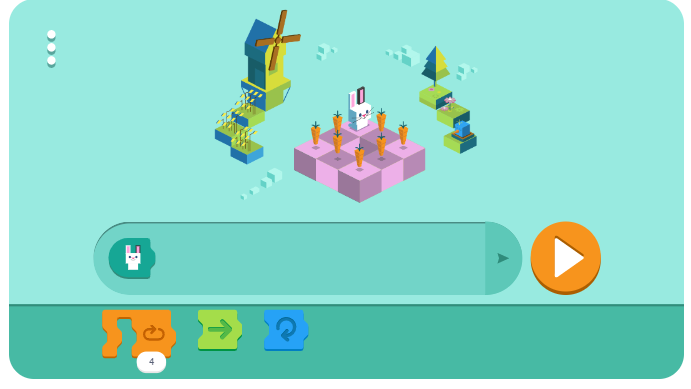
\includegraphics[width=105mm,scale=0.5]{images/nosoluce.PNG}
  \caption{Le niveau 4 du doodle}
  \label{fig:boat1}
\end{figure}

L'objectif ici est d'aider le lapin à manger toutes ses carottes en lui suggérant un chemin à prendre à l'aide de blocs de codes. Présentons plus en détail l'interface que l'on voit sur la figure 2.1 ; En bas nous avons les blocs de codes plus particulièrement la boucle en orange avec un indice '4' spécifiant que nous rentrons 4 fois dans la boucle, la flèche verte pour faire avancer le lapin et la bleu pour faire tournoyer le lapin selon la droite ou la gauche (sur la figure seulement à droite). Sur la ligne du dessus nous avons la ligne d'exécution du code où nous allons mettre nos instructions et enfin le bouton orange pour exécuter notre code. Ici nous avons donc un premier exemple de mise en place d'un algorithme en utilisant quelques notions basique comme la boucle et l'instruction. Avez vous trouvé la solution de la figure ci dessus ?

\newpage

\begin{figure}[!htb]
  \centering
  
\includegraphics[width=115mm,scale=0.5]{images/soluce2.PNG}
  \caption{Solution du problème}
  \label{fig:boat1}
\end{figure}

Le problème peut paraître assez simple pour nous mais est tout nouveau pour un enfant. Il faut aussi préciser que dans le cadre de ce jeu l'introduction à la boucle arrive au niveau 4 et que donc on accompagne intelligemment l'enfant pour la résolution des niveaux. Si vous voulez vous même essayer ce doodle le lien est disponible dans la bibliographie. Les niveaux suivants introduisent d'autres concepts comme la double boucle et demandent plus de réflexions. (Voir figure 2.3)

\begin{figure}[!htb]
  \centering
  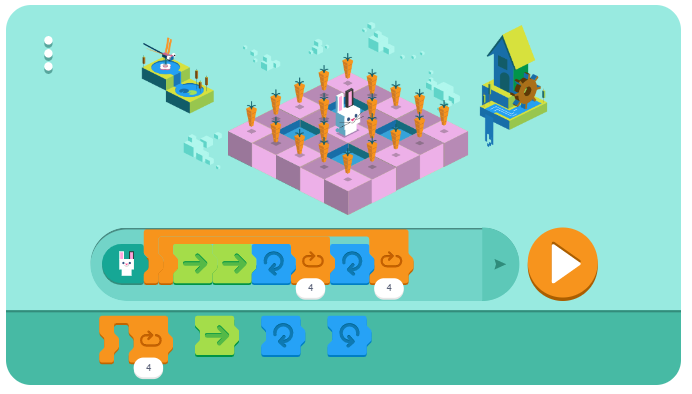
\includegraphics[width=115mm,scale=0.5]{images/soluce3.PNG}
  \caption{Niveau 5 et sa solution}
  \label{fig:boat1}
\end{figure}

Nous avons donc présenté ici une solution à la sensibilisation de l'algorithmique aux enfants. Cette dernière est ludique et accessible, l'enfant à la mainmise et la forme du jeu peut le pousser à s'investir davantage. Cependant, nous n'avons aucune donnée réelle sur l'efficacité de ce concept et l'expérience est plutôt éphémère puisque seulement 6 niveaux sont disponibles. Le doodle à été accessible 1 jour et nous n'avons pas de retour statistiques sur par exemple, est-ce que les utilisateurs ont aimé ? Quel âge avaient-ils ? Est-ce que cette expérience les a poussés à vouloir aller plus loin dans l'apprentissage de l'algorithmique ou de la programmation ? etc..

De ce fait, on ne peut pas interpréter scientifiquement et rigoureusement des hypothèses sur l'utilisation de ce doodle. Ce que l'on peut dire c'est que c'est une solution de familiarisation à l'algorithmique tant l'interface est simple et bien décrite.

\subsubsection{Le Langage Logo}

Ce que l'on peut noter par contre en partant de ce doodle, c'est que, comme dit plus haut, ce dernier fête le cinquantième anniversaire de l'encodage accessible aux enfants. Pour être plus précis, le doodle fête l'anniversaire du développement du langage Logo. \cite{12} Logo c'est un projet de chercheurs du MIT datant des années 1960 (la première version datant de 1967). C'est le premier langage de programmation pensé pour les enfants. Ce que l'on peut par exemple faire avec ce langage ce sont des dessins et des animations avec des instructions. Comme pour le doodle il y a les notions d'instructions et de boucle mais nous avons à faire ici à un langage à part entière. 

\newpage

Étant à la base un langage fait par des chercheurs il a amené à différentes études sur les résultats cognitifs des enfants utilisant ce langage. \cite{13}  La conclusion étant que, en plus de donner aux enfants des bases informatiques le langage Logo donne des résultats positifs sur des compétences scolaires. La reconnaissance de forme géométrique et de lettres, la différenciation de la droite et de la gauche et la créativité.

Nous ne savons pas si à partir de ses résultats nous pouvons lier la programmation informatique aux développement cognitifs énoncés mais en tout cas ce langage spécifique permet cela. Il faut dire que ce dernier est clairement construit autour de la création géométrique. Ce qui est sur c'est que cette étude démontre que Logo a un apport pédagogique. 

Pour tenter d'être plus concret sur Logo, ce dernier est aujourd'hui disponible sous de nombreuses formes avec des logiciels ou même sur navigateur internet. \cite{15} \cite{16} Il propose donc la possibilité de réalisation de formes géométriques (on donne des instructions de déplacement à une tortue) avec des concepts comme les boucles, les fonctions ou même la récursion. Il est doté de nombreuses primitives ou mots clés intuitifs (voir annexe) permettant l'exécution d'un programme. Il faut aussi préciser que ces mots clés sont traduits dans plusieurs langues dans un objectif de diffusion.

Prenons plusieurs exemples d'exécution de programmes à l'aide de l'outil en ligne cité précédemment.

\begin{figure}[!htb]
  \centering
  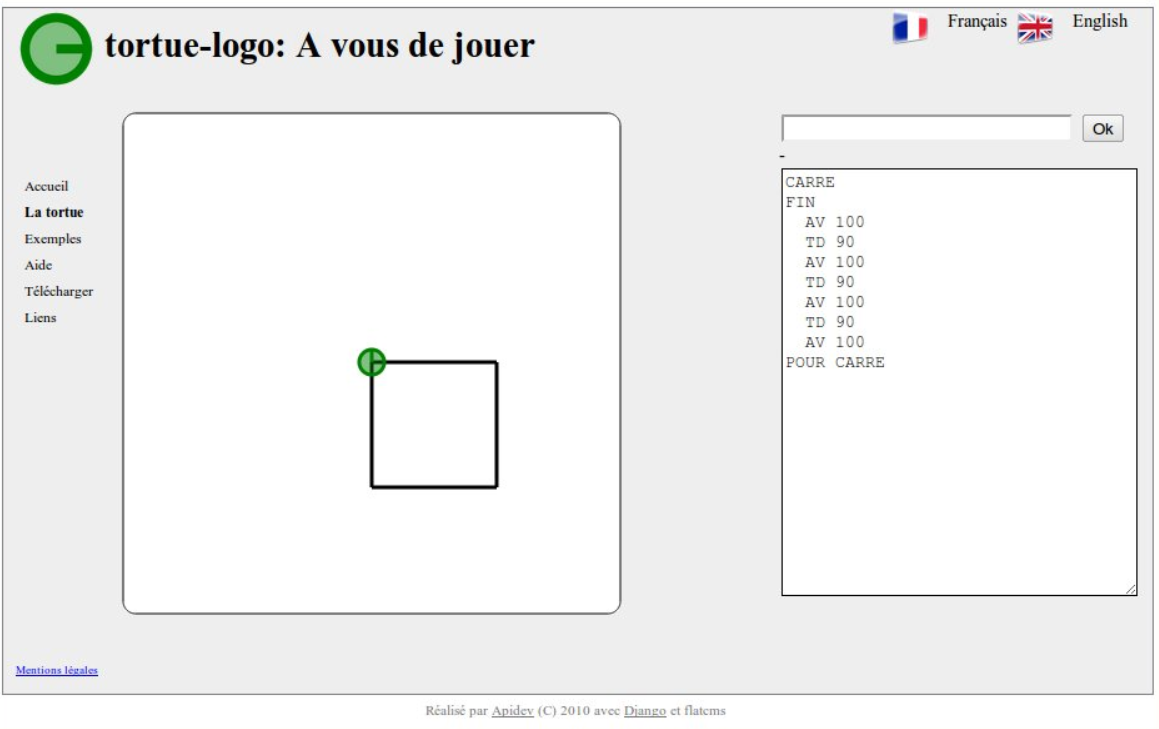
\includegraphics[width=105mm,scale=0.5]{images/logo1.png}
  \caption{Création d'un carré avec Logo}
  \label{fig:boat1}
\end{figure}

Voici un exemple de création d'un carré avec Logo, au vu des instructions passées et visibles à droite de la figure, nous pouvons créer un carré. Plus particulièrement, et avec l'aide de l'annexe, on peut voir que nous faisons avancer la tortue de 100 pas puis on change l'angle de 90 degrés puis on avance de 100 pas etc... Nous pouvons donc dorénavant construire le carré directement avec la commande que nous avons créée avec les mots clés FIN POUR. Cependant cette approche semble plutôt naïve puisque nous avons une redondance des instructions AV 100 TD 90. Par conséquent un moyen d'introduire le concept de boucle est d'utiliser le mot clé REPETE.

\begin{lstlisting}[frame=single]
POUR CARRE
  REPETE 4 [
    AV 100
    TD 90
  ]
FIN
\end{lstlisting}

A noter aussi qu'avec les mots clés FIN POUR on apprend aussi la notion de fonction. Comme dit juste avant, ce mot clé CARRE est maintenant réutilisable. Nous pouvons alors l'utiliser pour faire des formes géométriques plus complexes.

\begin{figure}[!htb]
  \centering
  \begin{minipage}[b]{0.45\textwidth}
    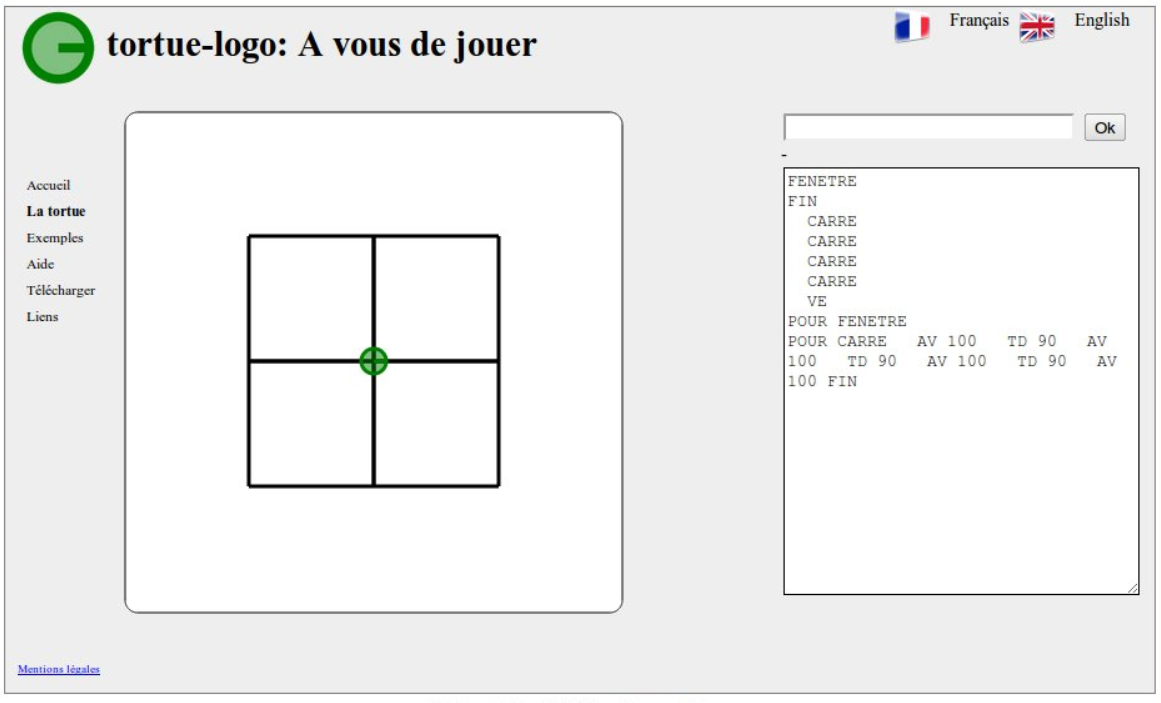
\includegraphics[width=\textwidth]{images/logo2.PNG}
    \caption{Dessin de 5 carrés}
  \end{minipage}
  \hfill
  \begin{minipage}[b]{0.45\textwidth}
    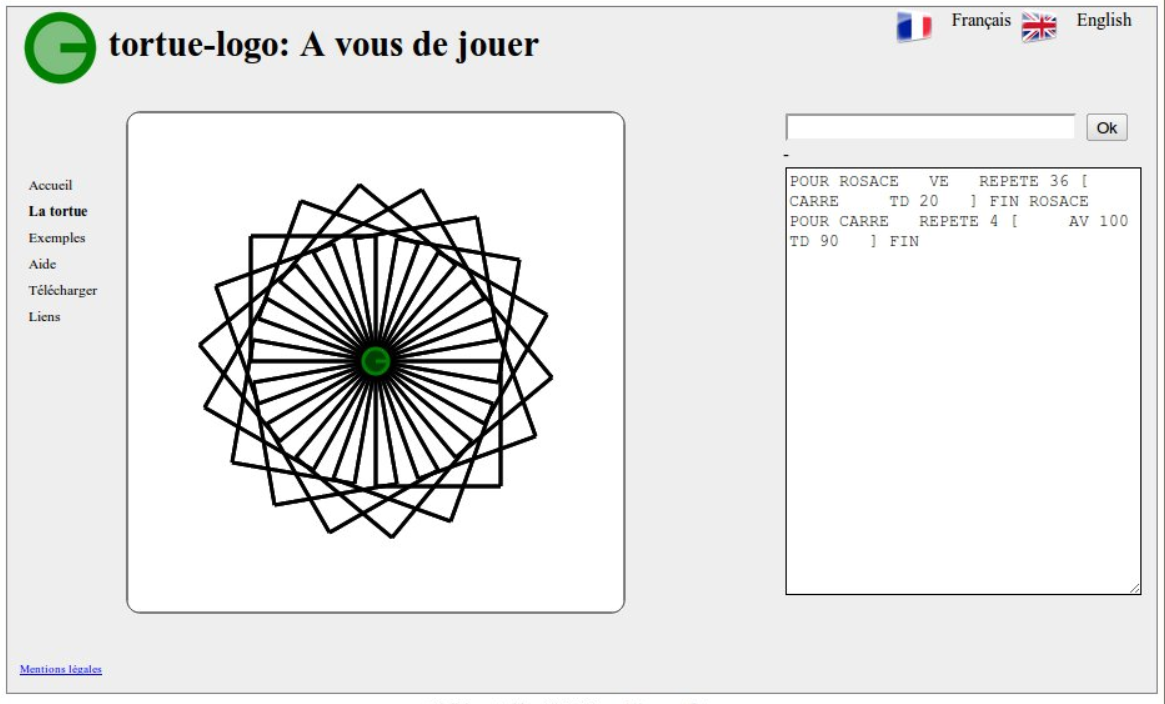
\includegraphics[width=\textwidth]{images/logo3.PNG}
    \caption{Dessin d'une rosace}
  \end{minipage}
\end{figure}

Voici donc un première exemple des possibilités de Logo. C'est donc un langage très accessible cependant il faut quand même un apport pédagogique extérieur d'une personne pour expliquer les bases (les primitives et la rédaction du code). Pour la suite, il est important d'introduire un nouveau mot clé : RECURSION. Comme son nom l'indique, ce mot clé sert à faire de la récursivité. En d'autre termes, c'est exécuter une action un nombre indéfini de fois en l'appelant de cette même action. Plus simplement, c'est s'appeler soit même pour une fonction informatique.

Ce concept semble être compliqué pour des enfants, mais c'est pourtant ce que des chercheurs de l'université de New York on voulu introduire \cite{14} dans leur document "Children's Mental Models of Recursive Logo Programs". 

Dans le contexte de cette étude, nous avons des enfants qui ont une expérience de 1 an avec Logo auquel nous leur demandons d'anticiper le résultat de programmes récursifs (comprendre ce qui va être dessiné). Il faut bien comprendre que ces enfants avaient donc des bases en itération, conditions, calcul et boucle. Il faut aussi savoir que le principe de récursion leur a été introduit.

\begin{lstlisting}[frame=single]
TO SHAPEB :SIDE
IFELSE :SIDE < 5 
  [STOP]
  
  [REPEAT 4 [FORWARD :SIDE RIGHT 90]
	RIGHT 90 FORWARD :SIDE LEFT 90
    SHAPEB :SIDE/2]
END
SHAPEB 80
\end{lstlisting}

C'est donc à partir d'un programme comme celui ci dessus que les enfants doivent anticiper le résultat. Les enfants doivent également expliquer comment le programme va procéduralement s'exécuter. Il pouvait notamment le faire à l'aide d'un crayon à papier sur une feuille et dessiner ce qui allait se passer. Plusieurs programmes comme celui ci-dessus étaient proposés sur des niveaux de complexité différents.

\newpage

Ce qu'il en ressort comme résultat est que tous les enfants (7 au total) ont donné des prédictions plutôt juste et avec peu de difficultés pour les 2 premiers niveaux de complexités. Pour le troisième (celui cité ci dessus) 2 enfants on eu des difficultés à comprendre la condition IF la confondant en une action pour guider la tortue. Malgré cela, le reste de leurs prédictions étaient juste. 
Cependant pour le niveau 4 de complexité (ci dessous) aucun enfant n'a trouvé la solution. 

\begin{lstlisting}[frame=single]
TO SHAPEB :SIDE
IFELSE :SIDE < 10 
  [STOP]
  
  [SHAPEB :SIDE/2
    REPEAT 4 [FORWARD :SIDE RIGHT 90]
	RIGHT 90 FORWARD :SIDE LEFT 90]
END
SHAPEB 80
\end{lstlisting}

Ce que l'on observe est que pour la complexité 3 nous avons une approche récursive terminale c'est à dire que la récursion est la dernière instruction à être évaluée, dans l'autre cas nous avons l'appel récursif qui est enchâssé dans le programme et donc logiquement moins évident à visualiser.

Malgré ces derniers résultats cela nous apprends quelque chose d'important face à l'apprentissage de l'informatique aux enfants. En effet, si ces derniers sont capables d'appréhender des concepts informatiques comme la récursion (avec condition d'arrêt), c'est alors clair qu'il est possible de leur apprendre des concepts plus simple (conditions, itération, variable etc...) à un jeune âge grâce à des solutions comme Logo.

\begin{figure}[!htb]
  \centering
  \begin{minipage}[b]{0.45\textwidth}
    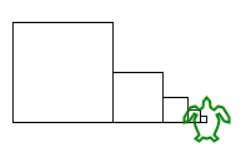
\includegraphics[width=\textwidth]{images/logo5.png}
    \caption{Dessin complexité 3}
  \end{minipage}
  \hfill
  \begin{minipage}[b]{0.45\textwidth}
    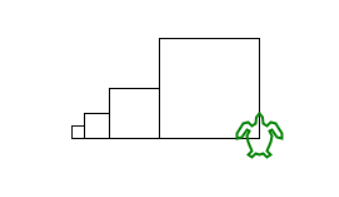
\includegraphics[width=\textwidth]{images/logo4.png}
    \caption{Dessin complexité 4}
  \end{minipage}
\end{figure}

\subsubsection{HANDS, Stagecast Creator, Visual Basic}

Pour partir dans un autre registre nous allons maintenant parler d'une étude réalisée par des chercheurs de l'université de Taiwan \cite{2} qui non seulement étudient l'impact de l'apprentissage de concepts informatiques différents mais également le retour des enfants sur leur apprentissage (leurs sentiments, si ils ont aimé) ainsi que le retour des parents. Pour cela des données ont été recueillies et analysées sur les différents concepts.

\newpage

Dans cette étude nous avons 81 enfants de 10 à 12 ans auxquels nous apprenons à utiliser 'Stagecast Creator', 'HANDS' et Visual Basic afin de créer des jeux simples et des animations. Le but et l'idée introductive de ce papier est qu'il semble important d'introduire des concepts informatiques à l'école élémentaire mais que nous n'avons pas forcément les bons outils et que nous voulons tester des nouvelles manières de faire de façon ludique. C'est dans ce but et avec cet essai pilote que cette étude à été faite. Parmis la population d'enfants, seulement 3 avaient des expériences avec la programmation avant avec JavaScript, Logo et Lego Mindstorms. Les 3 technologies citées avant représentent 3 techniques différentes de programmation. Dans un des cas nous n'avons pas besoin d'écrire du code (Stagecast) dans le deuxième cas nous avons besoin d'écrire des instructions proches du langage parlé (HANDS) et dans le dernier cas nous avons à écrire du code dans une syntaxe précise (Visual Basic).

Ce qui est déjà intéressant de noter est la montée de difficulté croissante qui accompagne sûrement mieux l'élève d'un point de vue pédagogique. Il est moins risqué de perdre l'élève en partant d'un point de vue ou l'on doit par exemple créer ses conditions de façon seulement graphique pour atteindre un niveau où ces conditions doivent être mentionnées dans une syntaxe particulière. 

Pour Stagecast Creator cette vidéo \cite{17} explique très bien le logiciel, comment marche les règles ou conditions et un exemple de jeu que l'on peut faire avec. On observe bien dans cette vidéo que tout ce qui est fait ne nécessite pas une ligne de code mais introduit tout de même des concepts informatiques. Avec cette façon de faire nous avons très peu de chance de perdre un élève sachant que tout est visuel.

Pour HANDS, nous utilisons donc des phrases proche de la langue pour décrire des instructions et les interactions entre les personnages.

\begin{figure}[!htb]
  \centering
  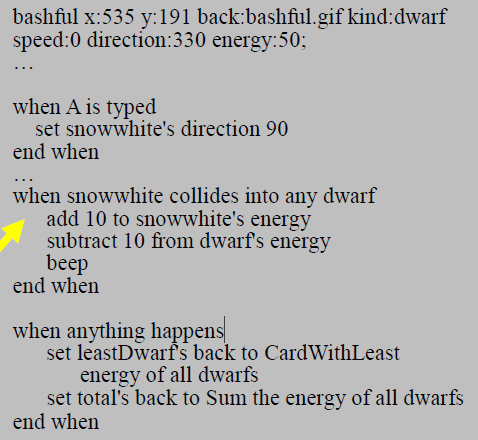
\includegraphics[width=60mm,scale=0.5]{images/hands.png}
  \caption{Exemple d'instructions sur HANDS}
  \label{fig:boat1}
\end{figure}

Voici donc ci-dessus un exemple d'instruction sur HANDS. Nous observons que ces dernières sont facilement interprétables même sans la présence de l'interface graphique, qui est une représentation simple de Blanche Neige et les sept nains (visible sur le papier de recherche). Ce que l'on peut noter sur HANDS est que le logiciel semble être aujourd'hui plus utilisé tant il est introuvable sur le web. C'est, je pense, un problème important si l'on veut trouver des solutions pédagogiques sur le long terme parce cette expérience ne serait plus réalisable aujourd'hui. Si l'on veut mettre en place un système pédagogique il faut être sur de la longévité et de la capacité à durer dans le temps d'un projet/logiciel.

Enfin la dernière phase de l'expérience était la réalisation d'une calculatrice avec Visual Basic, le langage de Microsoft. Ce langage est destiné notamment à créer des applications avec l'interface graphique des programmes Windows. On peut, en effet, se dire que ce genre de langage n'est pas adapté pour les enfants étant donné que des professionnels utilisent eux même Visual Basic. Cependant avec l'accompagnement fait sur la programmation à l'aide des logiciels précédents plus 'haut niveau' les élèves ont pu appréhender un langage comme Visual Basic plus facilement. Surtout, au vu des données récoltées et des retours des élèves cette expérience à été efficace et bénéfique pour eux.

Cette expérience a pu notamment mettre en valeur deux choses importantes : l'apprentissage de l'informatique est accessible aux enfants de cette âge, ça leur plaît et ça plaît également à leurs parents. Si l'on sort les chiffres de l'étude nous avons des données pour chaque partie de l'expérimentation (c'est à dire les 3 phases). En résumé il est intéressant d'observer que les meilleurs notes sont données à Stagecast et Visual Basic (le second semblant pourtant moins accessible). Il est encore plus intéressant de voir que Visual Basic est la phase préférée des élèves pour 56.9\% .

Quant aux parents, la plupart d'entre eux ont notifié que leurs enfants avaient hâte de se rendre en cours de programmation et passaient également du temps chez eux (plus de 1 heure) à travailler dessus. En plus de cela, les enfants étaient fiers de leur montrer leurs travaux informatiques et énonçaient également qu'ils étaient intéressés d'en apprendre plus sur l'informatique.

Ce qu'il faut retenir de cette expérience c'est surtout que l'apprentissage de l'informatique est loin d'être inaccessible aux enfants, c'est en plus une matière qui peut se révéler prenante si elle est présentée d'une manière ludique. Étant donné que dans l'expérience, nous avons un résultat concret et amusant (en tout cas pour les jeux), les chiffres énoncés précédemment me semblent cohérents dans l'hypothèse faite avant l'état de l'art : le ludique et le contexte d'apprentissage sont primordiaux.

\subsubsection{Sonic Pi}

Dans les parties précédentes, nous avons vu qu'il était primordial d'avoir un bon environnement pour apprendre aux enfants la programmation dans des conditions optimales. L'environnement comprend donc l'équipe pédagogique (il faut avoir soit des enseignants d'informatique soit des professeurs préparés à l'apprentissage dans ce domaine). Même si nous pouvons penser que l'informatique peut être appris en autodidacte et qu'une grande partie de l'apprentissage se fait par la pratique, pour les enfants le contexte est différent. Les enfants sont donc réceptifs à l'apprentissage de la programmation ou à l'algorithmique mais il nous faut donc ce contexte comme nous avons vu avec Logo. C'est dans cette idée que s'inscrit Sonic Pi. L'idée de Sonic Pi est de proposer un environnement de développement avec son langage dédié et orienté apprentissage. L'idée principale est de proposer l'apprentissage de la programmation avec la musique. Même si l'on est pas tous forcément mélomanes, ce contexte est clairement ludique car le résultat de notre code (qui produit donc de la musique) est un résultat concret. Différents projets on été fait avec Sonic Pi, par exemple recréer Aerodynamic de Daft Punk \cite{18} . Cependant ce qui nous intéresse ici c'est l'apprentissage avec Sonic Pi et c'est notamment ce qu'ont étudié certains chercheurs de l'université de Cambridge dont fait partie Samuel Aaron, le créateur de Sonic Pi. Ils ont notamment étudié l'utilisation de Sonic Pi dans l'éducation, la pédagogie de la programmation ainsi que les performances de cette utilisation. \cite{19} \cite{20}

Dans un premier temps nous allons présenter les bases de cet environnement de développement pour bien comprendre de quoi on parle et expliquer en quoi cette solution s'inscrit bien dans un contexte d'apprentissage.

\newpage

\begin{figure}[!htb]
  \centering
  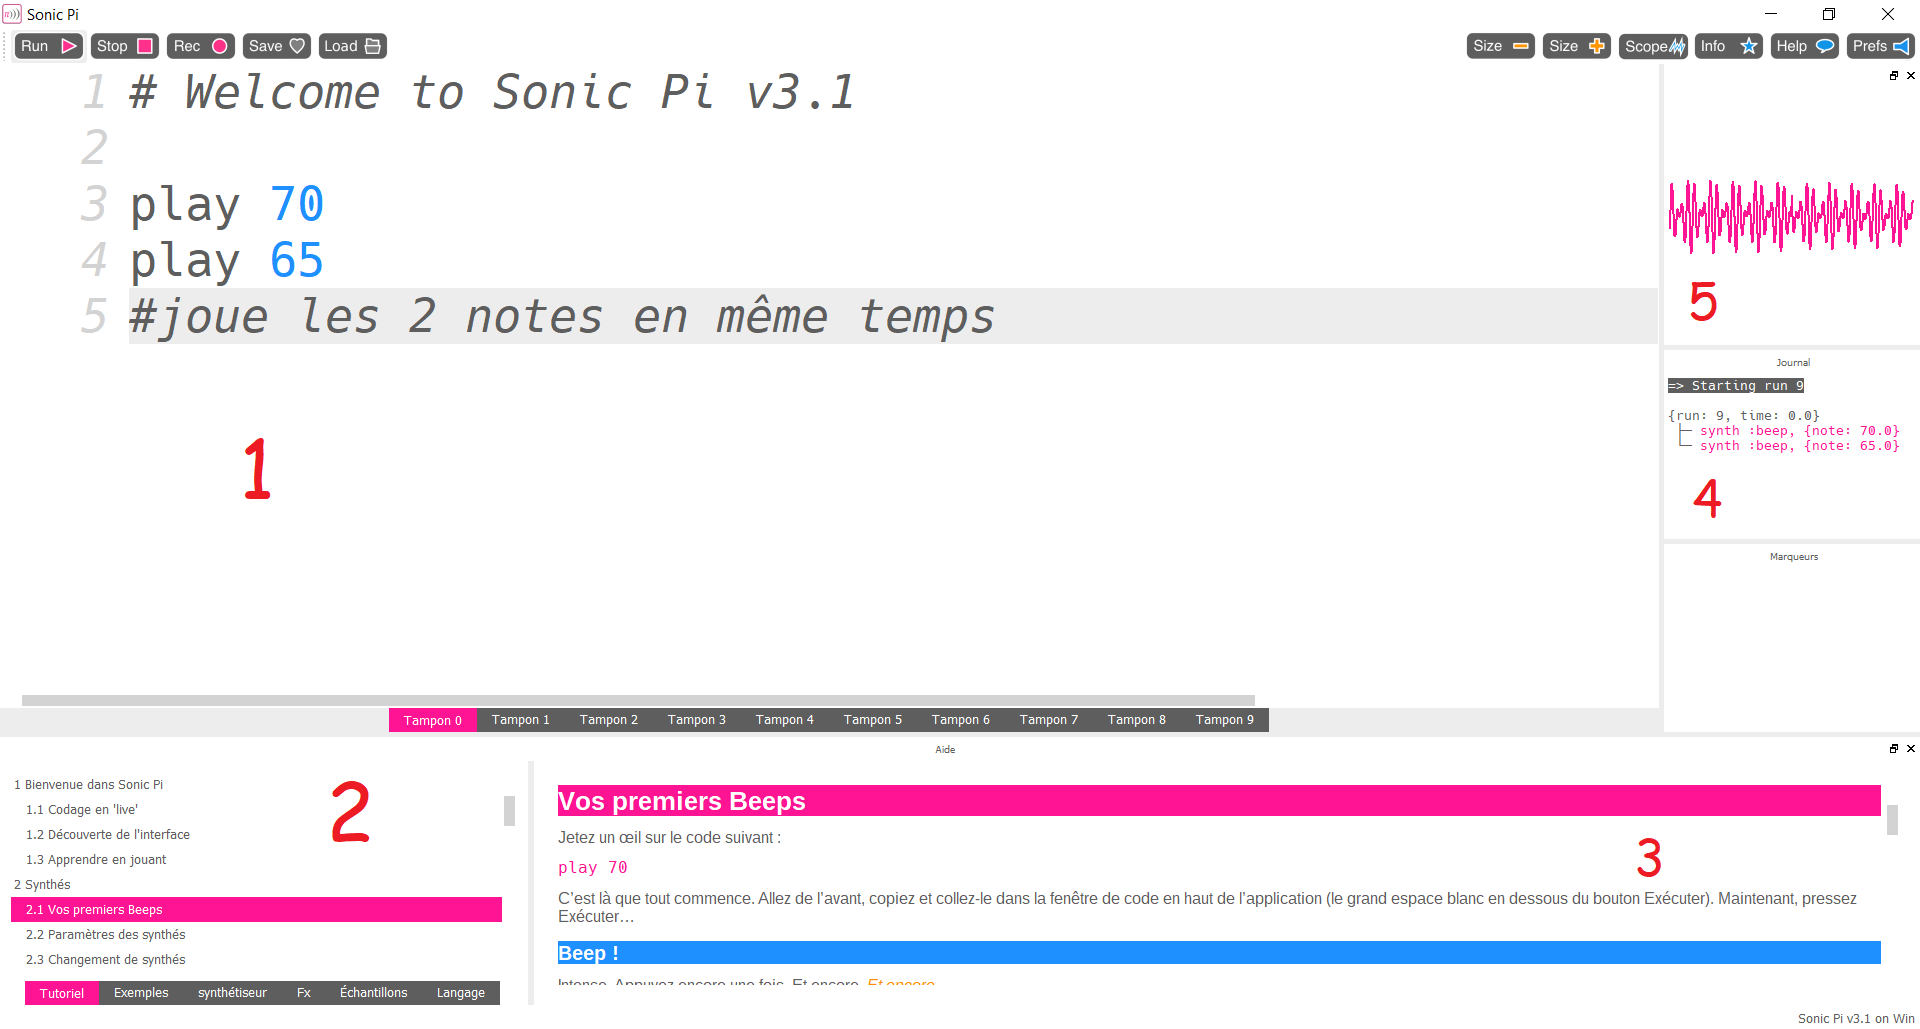
\includegraphics[width=110mm,scale=0.5]{images/sonic_pi_ide.png}
  \caption{L'IDE Sonic Pi}
  \label{fig:boat1}
\end{figure}

En se fiant aux numéros sur la figure, on peut rapidement présenter le logiciel comme le 1 étant la zone de saisie de texte (la ou l'on écrit le code) par exemple dans la capture d'écran on joue 2 notes (les instructions play 70 et play 65). Pour expliquer brièvement, plus le nombre passé en paramètre de play est petit plus le son est grave car on s'associe au système du piano (play 40 on joue la 40ème note du piano). Des exemples de fonctions et instructions de Sonic Pi sont données en annexe. Le 2 et le 3 sont des tutoriels d'introduction à Sonic Pi, le menu étant le 2 et le descriptif le 3. Le 4 est le journal d'exécution du programme et le 5 est la fluctuation ondulatoire du son.

Ce que l'on peut noter tout de suite, c'est la volonté pédagogique à travers ce projet étant donné que tout un tutoriel est fait (point 2 et 3) en s'adressant à de parfaits novices en programmation. De plus, le langage et l'IDE (pas de création de projets, tout de suite prêt à l'emploi) est également orienté pour être simple et disponible au début. Cependant si on veut aller plus loin dans le langage en étant enfant, il me semble important d'avoir un encadrant car même si c'est ludique on peut vite entrer dans des concepts plus compliqués qui nécessitent de l'attention.

Ce qui est important de préciser pour Sonic Pi est que le langage utilise le "Live Coding" ou programmation à la volée, le programme est directement modifiable lors de l'exécution ! C'est une technique de programmation beaucoup utilisée lors de création de musique via ordinateur afin de voir l'évolution direct de l'apport que l'on fait au code. Bien qu'il existe des langages similaires pour ce genre de réalisation (ChucK, FAUST, ou un exemple concret \cite{21} ...), Sonic Pi semble être le plus orienté pédagogie puisqu'il a été à la base conceptualisé pour cela et il est également gratuit donc facilement diffusable dans un contexte éducatif.

Si on se réfère aux articles précédemment énoncés sur Sonic Pi notamment \cite{19} il a été expérimenté un schéma de cours à suivre avec Sonic Pi en 5 heures. Pour Aaron et ses collègues, la découverte et pratique créative associées au "Live Coding" fonctionnent ensemble et permettent une meilleure expérimentation. Ils ont développé donc le schéma suivant en 5 leçons de 1 heure chacune.

Dans un premier temps les élèves apprennent l'architecture basique de l'ordinateur, la mémoire, l'entrée sortie, ce qu'est le programme c'est à dire les séquences du programme ainsi que la déclaration écrite des instructions et leurs ordres dans le programme. Avec le "Live Coding" il est d'autant plus facile d'apprendre les conséquences d'un changement d'ordre des instructions d'un programme étant donné que ce changement est directement observable ou plutôt audible.

Dans la deuxième leçon, les élèves apprennent la syntaxe des programmes, les erreurs de mauvaise syntaxe qui doivent être débuguées, les structures de programmation (boucle etc) ...

\newpage

Dans la troisième, les conditions sont abordées, la condition simple ainsi que les branches de décisions. Il est aussi abordé la randomisation, notion intéressante dans le cas de programmes créatifs et musicaux (jouer une suite de notes d'une gamme au hasard). En plus de l'explication de l'importance de bien structurer son programme il y est aussi appris aux enfants à comment utiliser des commentaires dans le code (expliquer une partie de code complexe et/ou intéressante).

Les algorithmes sont introduits dans la quatrième leçon ainsi que les structures de données (liste, etc...)

Le notion de concurrence est abordée dans la dernière leçon c'est à dire le multi-tâche avec différents threads.

L'observation qui a été faite sur Sonic Pi est que au début les concepteurs de Sonic Pi et les chercheurs pensaient que la musique était un juste un cadre pour guider l'apprentissage. Il en est ressorti que finalement cela à eu un impact beaucoup plus important :

\begin{quote}
    "\textit{The
music not only provided a rich set of analogies with which to represent the computing
constructs. It also enabled a level of engagement that the collaborating teacher had not
observed in some students. Mid-lesson demonstrations of the music produced so far provided
much interest across the classroom due to the huge diversity of the musical outputs
being created and the performative nature of the delivery. This often led directly to a lot of
spontaneous knowledge sharing. Finally, a lot of the students were treating Sonic Pi as a
musical system rather than a programming language-learning tool.}"

\end{quote}

Source "International Journal of Performance Arts and Digital
Media : Volume 12, 2016"

Par conséquent, il a été observé que l'implication des élèves était importante grâce à l'environnement proposé par Sonic Pi. Finalement les élèves étaient très participatifs aux cours et posaient, sans se rendre compte, des questions en rapport avec l'informatique (Comment je répète cette ligne de basse ?  Comment je fais pour jouer cette mélodie au même moment que la ligne de basse ?). Ces questions qui font par exemple référence aux boucles ou à la concurrence. Finalement la notion de concurrence peut être abordée pour des enfants alors que ce sont normalement des concepts vus en université. Il est intéressant de noter qu'un concept comme la concurrence peut être abordé de manière ludique !

\subsubsection{Le drag-and-drop}

Comme énoncé dans l'introduction, le système de drag-and-drop ou glisser-déposer est beaucoup utilisé dans les langages de programmation pédagogiques. Nous prendrons ici deux logiciels en exemple : Alice et Scratch.

Pour présenter brièvement Alice, c'est un logiciel datant de 1998 développé par l'université Carnegie-Mellon. On utilise le système de drag-and-drop pour créer des animations. En fait, on assemble des instructions avec une interface graphique intuitive qui nous permet de créer des animations. Comme pour les exemples précédents, l'objectif est de transformer l'informatique comme quelque chose d'amusant et ludique, on fait ici aussi appel à l'esprit créatif de l'enfant sachant qu'il peut créer ses propres histoires avec les animations. Il n'y a ici donc pas de syntaxe complexe. Les utilisateurs peuvent programmer en glissant-déposant des briques d'instructions qui représentent des structures logiques. Contrairement à Scratch, Alice propose une représentation en trois dimensions du résultat du programme.

\newpage

\begin{figure}[!htb]
  \centering
  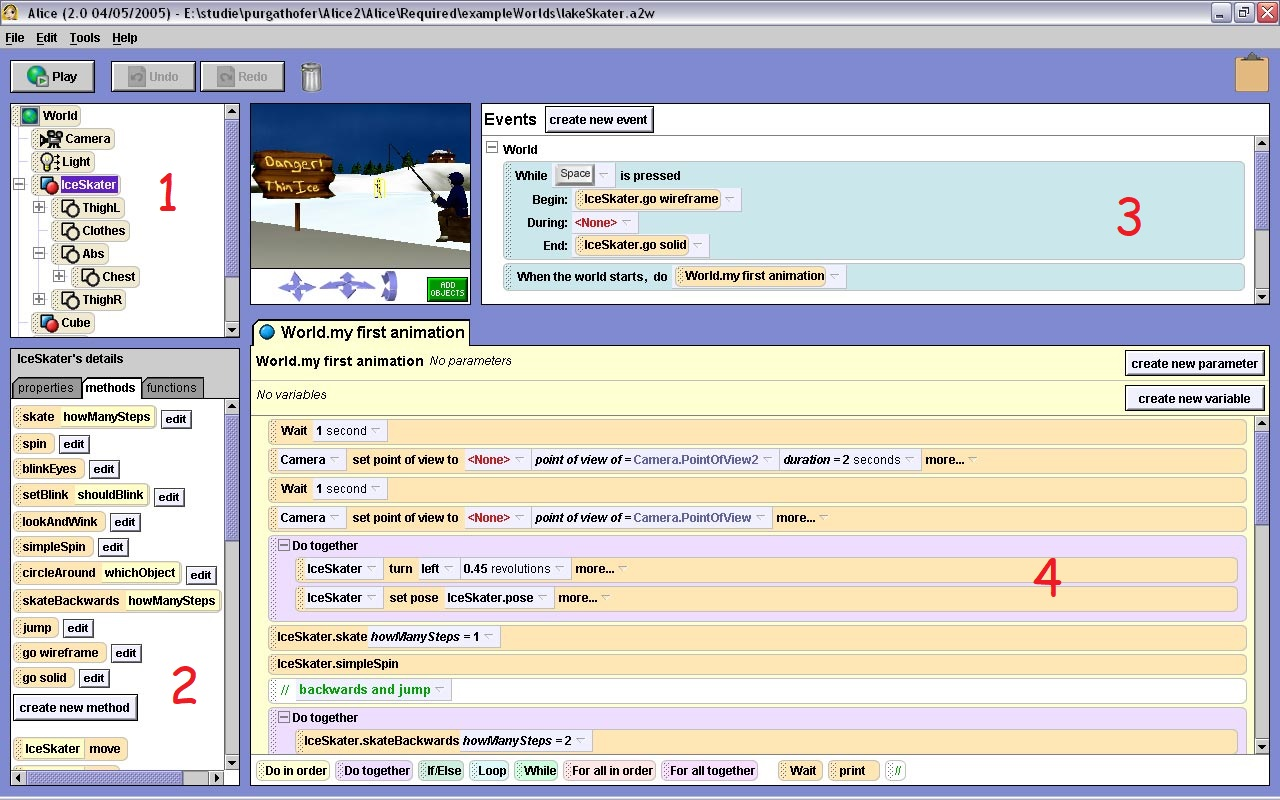
\includegraphics[width=150mm,scale=0.5]{images/alice-ide.jpg}
  \caption{L'IDE Alice avec un exemple d'animation}
  \label{fig:boat1}
\end{figure}

La figure ci-dessus nous présente l'environnement de développement, il existe une autre interface sur le logiciel pour placer les objet sur une scène (leur position inclinaison etc...). Que ce soit avec une scène 2D ou 3D, comme cela n'a pas vraiment de rapport avec la programmation nous allons plutôt parler de la partie encodage de l'animation. Dans la zone 1, nous avons la liste des objets de la scène présentée sous forme d'arbre. (L'objet IceSkater contient ThighL, Clothes etc...). Dans la zone 2, nous avons un panneau qui présente les actions ou méthodes utilisables par les objets de la scène par exemple pour qu'ils puissent interagir entre eux ou avec l'environnement. La zone 3 représente le programme ou l'exécution du code. Dans l'exemple ci dessus on peut voir que l'on appelle la fonction que l'on a définie dans la zone 4 qui est le panel d'édition de code ou l'on écrit notre programme. C'est dans cette zone 4 qu'il y a le système de drag-and-drop avec les différents types de briques en bas de la capture d'écran. Avec ce système on peut donc créer ses animations, histoire, suivant les instructions logiques que l'on a défini, de nombreux exemples sont disponibles ici : \cite{22}

D'un point de vue éducation et recherche, Alice à été testé dans des écoles et il en ressort différentes statistiques. Notamment, les élèves qui ont eu une approche d'apprentissage de Alice suivi par JAVA avaient de meilleurs résultats que ceux qui ont fait l'apprentissage sans logiciel éducatif comme Alice (84.96\% de réussite en moyenne contre 60.8\%). \cite{23} Il faut aussi préciser que Alice permet de convertir ses fichiers en Java ce qui permet une meilleure approche du langage. Dans ce cas, on s'éloigne cependant des enfants car cette étude est pour des étudiants, mais cela prouve l'utilité d'une approche ludique avant un concept concret que ce soit enfant ou étudiant. Il existe aussi d'autres études similaires où les notes moyennes sont passées de C à B en informatique. Il y a aussi des meilleures statistiques de présence aux leçons et une meilleure motivation des élèves parmi ceux qui ont participé à l'expérimentation avec Alice que les autres. \cite{24} Enfin, une autre étude concernant cette fois les enfants montre que ces derniers ont abordé des niveaux d'abstraction et de modélisation, des structures de contrôle et également géré des évènements dans leurs animations avec en général beaucoup de succès. \cite{35}

\newpage

Concernant Scratch, il est semblable à Alice mais plus récent. Il propose également un système de drag and drop intuitif et accessible qui permet de faire des animations. Ici les animations sont par contre en 2D. Cependant il semble encore plus accessible que Alice tant que aujourd'hui FranceTv Éducation a créé des ressources d'apprentissages avec Scratch pour les élèves de primaire (de ce1 à cm2). \cite{25}


\begin{figure}[!htb]
  \centering
  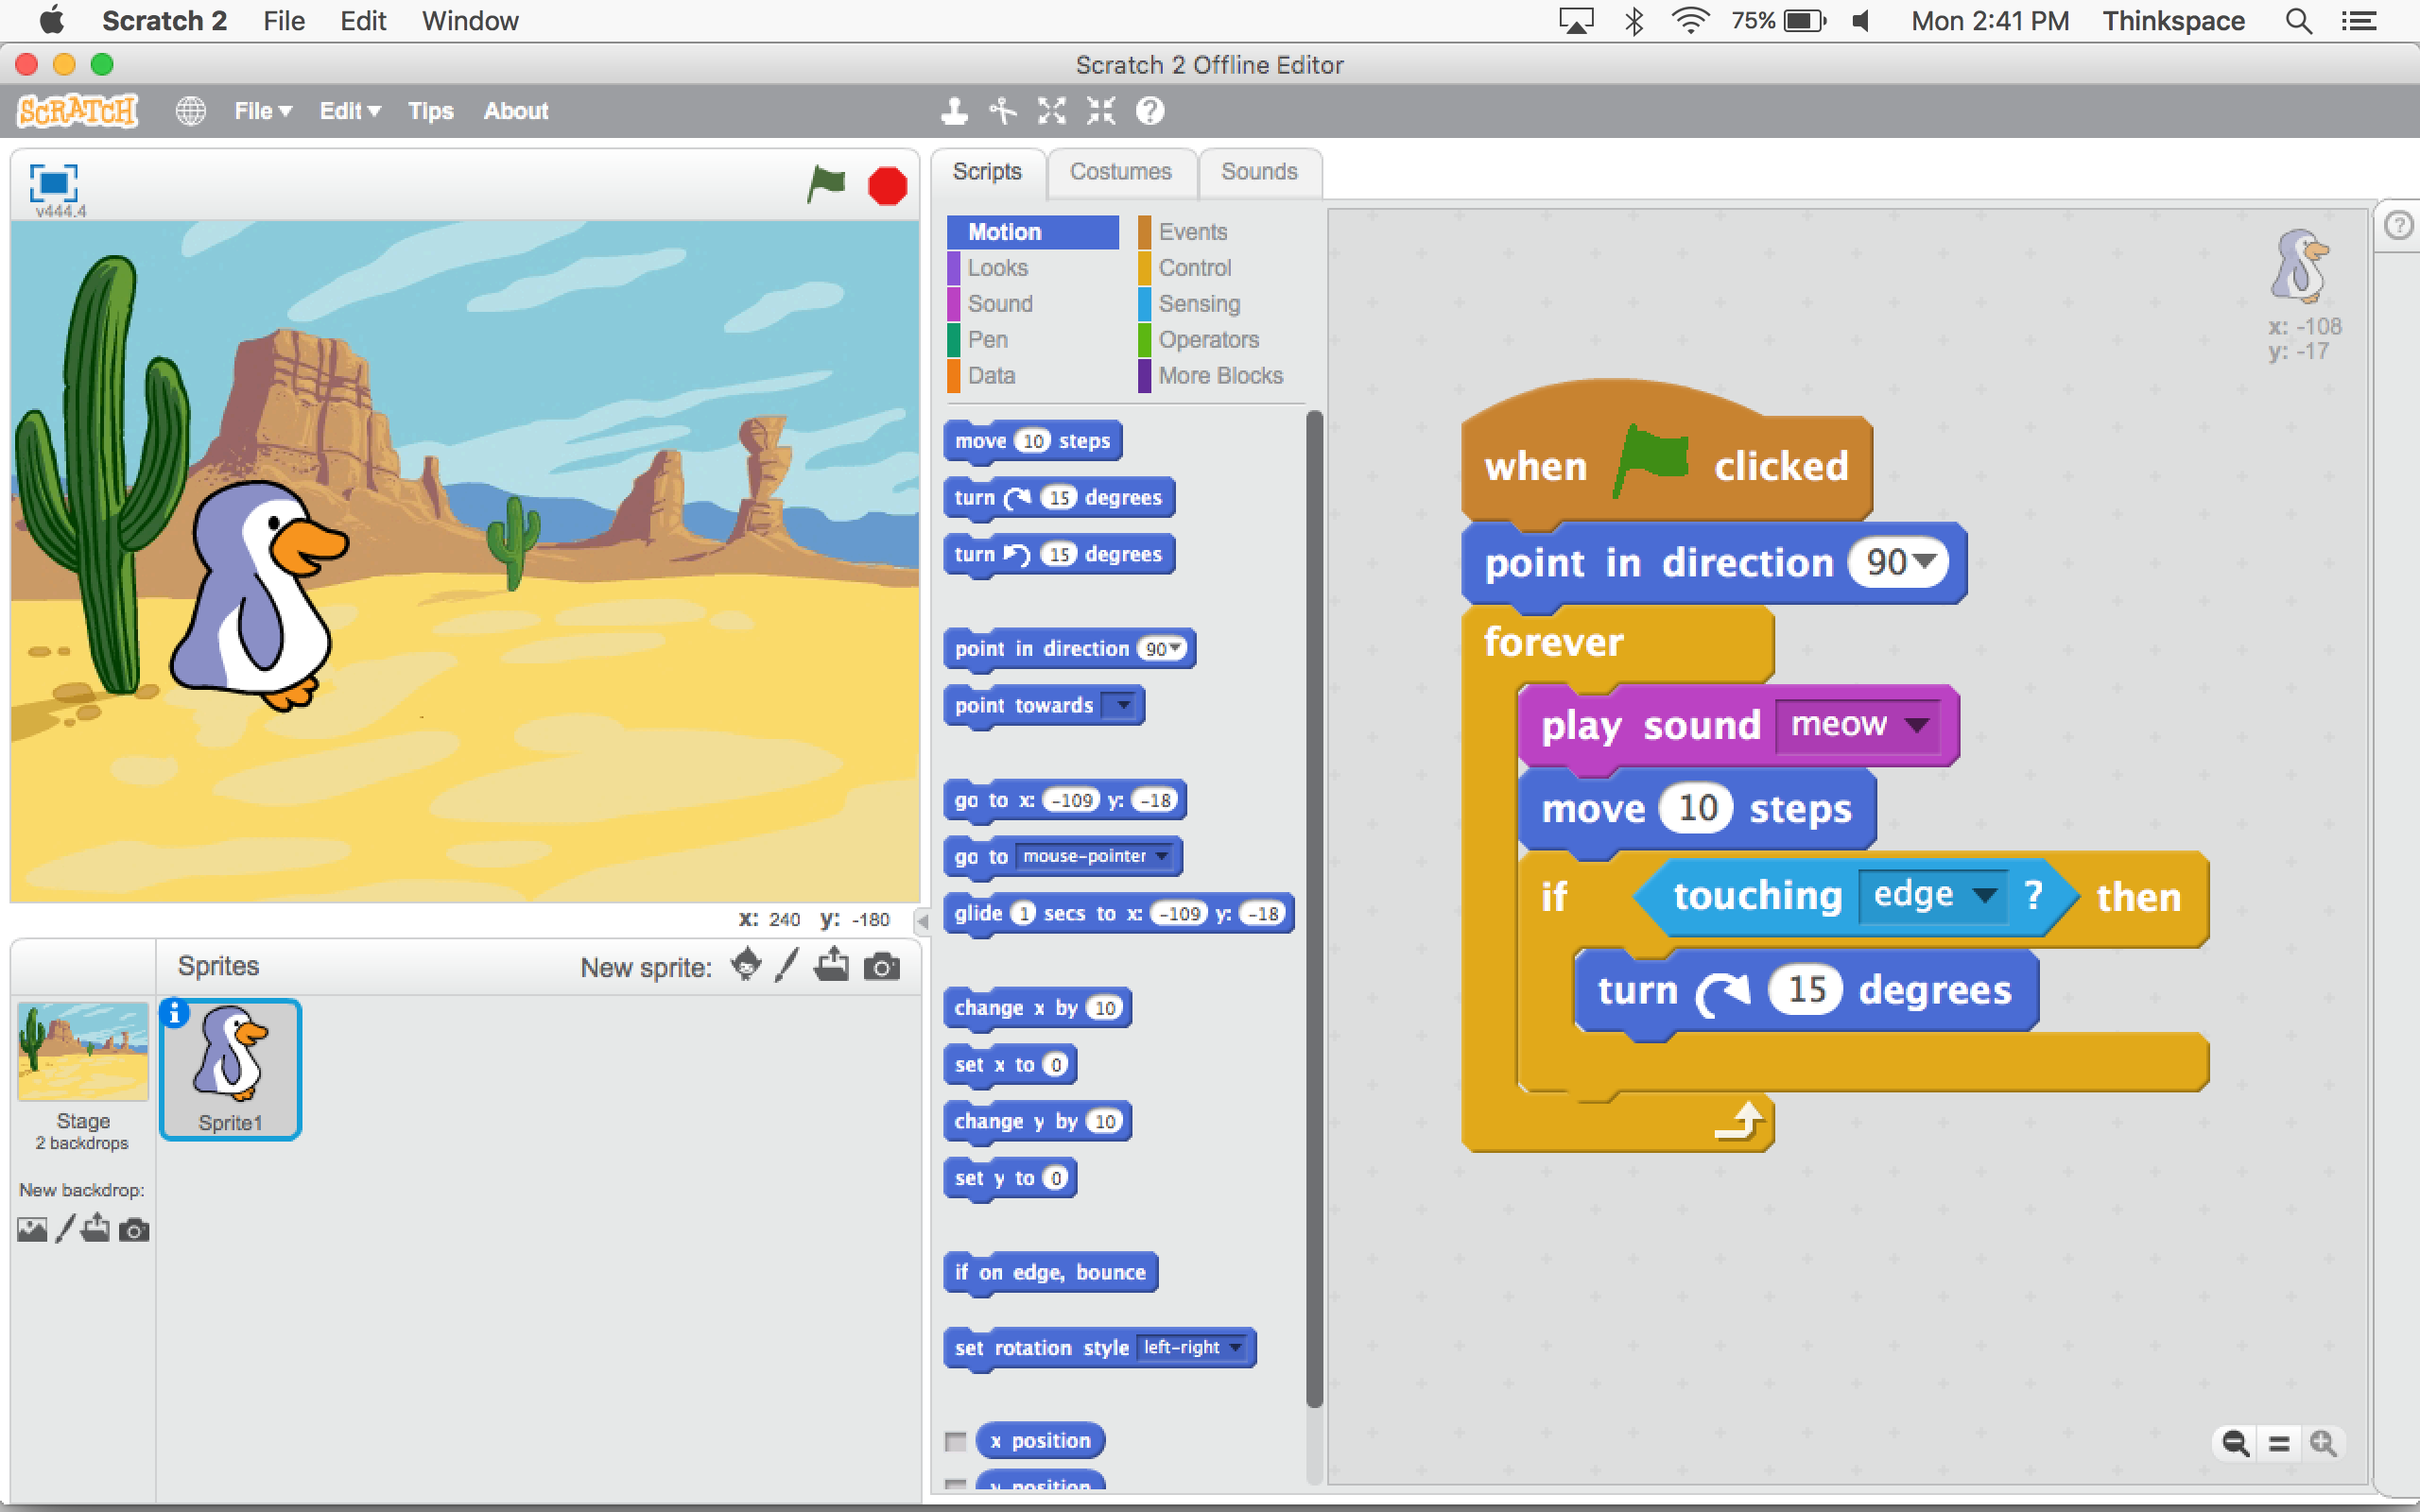
\includegraphics[width=125mm,scale=0.5]{images/scratch-ide.png}
  \caption{L'IDE Scratch dans sa version 2.0}
  \label{fig:boat1}
\end{figure}

La configuration est semblable à Alice, nous avons une partie où l'on a une suite d'instructions que l'on peut déposer à droite sur le panel d'édition de code. Les instructions sont imbriquées les unes dans les autres un peu comme on a pu le voir précédemment pour le doodle de Google. Il y a notamment la présence de conditions, boucles, instructions ... 

En France, dans les sujets 0 du diplôme du brevet (collège) on fait notamment référence à Scratch pour des notions de codage et de programmation. \cite{26} On peut donc imaginer que ce logiciel va être éventuellement utilisé comme une solution de la sensibilisation à l'informatique dans les collèges.

L'utilisation de Scratch à notamment été étudié \cite{27} pour voir si il était utilisable dans l'enseignement. Dans cette étude on est dans un cas similaire à une étude sur Alice ou on passe d'un apprentissage de Scratch à Java (et donc on a plus affaire à des étudiants). Une autre étude donne des résultats positif sur l'utilisation de Scratch avec des enfants, notamment sur leur motivations et leur ressentis face à l'apprentissage. \cite{36} Une autre étude encore donne une bonne idée de l'utilisation des différentes briques sous forme de pourcentage. Sachant que chaque brique peut aborder des concepts informatiques différents et que la plupart sont utilisées à plus de 50\%. Il y a aussi des statistiques intéressantes en fonction du sexe de l'enfant. On remarque notamment que les filles semblent mieux se débrouiller en parallélisme et synchronisation. \cite{37}

En conclusion le drag-and-drop semble être une solution efficace mais nous avons fait cette analyse sur seulement 2 logiciels. Outre cela, il est clair que l'idée des environnements drag-and-drop sont très accessibles et facilement compréhensibles surtout si il y a un travail d'intuitivité sur le logiciel comme c'est le cas pour nos deux exemples (parcours utilisateur etc ... Surtout que ce parcours utilisateur doit être pensé pour des enfants).

\newpage


\subsection{L'apprentissage manuel}

L'apprentissage manuel désigne une expérience d'apprendre l'informatique sans la machine. Si l'on compare cette idée avec la partie précédente, l'expérience est plus éphémère, elle s'adresse également à un public jeune. Cet apprentissage manuel est souvent effectué par le jeu et le rend très accessible, il est également 
simple à mettre en place (pas d'installation etc...) et ne nécessite pas d'interfaces payantes. L'idée ici, c'est donc apprendre l'informatique sans informatique ! Un concept qui peut paraître étonnant mais néanmoins intéressant. Si l'on peut penser que, malgré les parties précédentes, l'informatique est inaccessible aux enfants, avec ce genre de solutions on ne peut plus le nier !

J'ai été personnellement confronté à ce genre d'apprentissage à la fête de la science sur le campus de Jussieu à Paris. Durant la fête de la science, différentes activités sont proposées pour différents domaines scientifiques et notamment l'informatique. Nous avions alors la présence d'un jeu de tri, donc comprendre comme le tri informatique, où des participants partaient d'une ligne où ils étaient "non trié" (ils ont sur eux un panneau avec un nombre) et arrivaient sur une autre ligne où ils finissaient triés. Pour mieux comprendre, si l'on a une liste de participants en ligne avec chacun un panneau où ils sont distribués comme ceci : [5, 2, 4, 1, 3], à la fin du jeu ils seront sur la ligne finale alignés comme ceci : [1, 2, 3, 4, 5] et donc triés. On peut notamment voir un déroulement de ce jeu ici \cite{28} .

\begin{figure}[!htb]
  \centering
  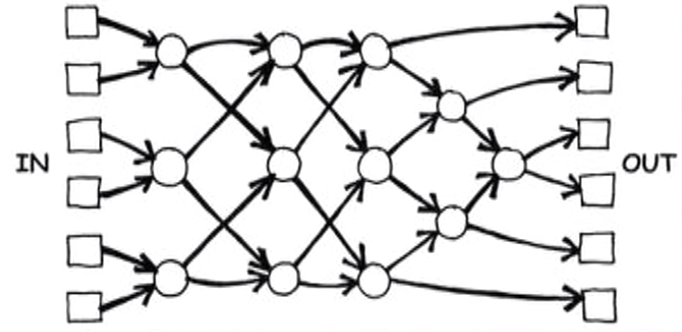
\includegraphics[width=115mm,scale=0.5]{images/tri.PNG}
  \caption{Le plateau du jeu de tri}
  \label{fig:boat1}
\end{figure}

Maintenant que nous avons expliqué l'entrée sortie du jeu, nous pouvons commenter le fonctionnement du tri avec la figure ci dessus. Les participants commencent donc à gauche en étant mélangés et finissent triés à droite. A la première étape ils se dirigent vers le premier rond en suivant leur flèche respective et à l'étape du rond ils comparent leur nombre avec l'autre participant (nombre plus petit, plus grand ?). Si on est un nombre plus grand, on va vers la droite sinon vers la gauche. En comparant ainsi tous les nombres on finit par être trié à l'étape finale. Ce jeu apprend notamment des principes de base de tri informatique mais l'expérience est courte, surtout par exemple à la fête de la science.

Cependant, il existe différents projets d'apprentissage par le jeu de loisir comme celui-ci qui permettent de perpétuer l'expérience plus longtemps comme avec le "Computer Science Unplugged" qui a pour objectif d'apprendre l'informatique avec les puzzles, le jeu, les histoires et donc sans ordinateur ! \cite{29} Le projet CS Unplugged a notamment une vocation internationale, bien qu'il ai été développé en Nouvelle-Zélande, il y a un désir d'internationalisation (traduction dans différentes langues) et des feuilles de routes pour une utilisation en classe avec des explications de comment procéder à l'attention des professeurs. Tout est décrit sur le site officiel. \cite{30}

\newpage

Parmi les jeux que propose le programme CS Unplugged il y a notamment le "Orange Game". Ce jeu propose de s'initier aux notions de blocage par exemple présent en concurrence. Les règles sont assez simple, on a un nombre x d'enfants et chacun d'entre eux possède un t-shirt de couleur différent, il y a aussi le même nombre x de fruits différents et ils sont tous présents par paire sauf un. Chaque enfant doit tenir dans ses deux mains les deux fruits de la couleur de son t-shirt sauf celui où il y a un seul fruit où il aura alors une main libre. Au début du jeu, les fruits sont distribués de façon aléatoire dans les mains des enfants et ils doivent alors résoudre le problème. On peut passer un fruit seulement dans une main libre et à un de ses voisins.

\begin{figure}[!htb]
  \centering
  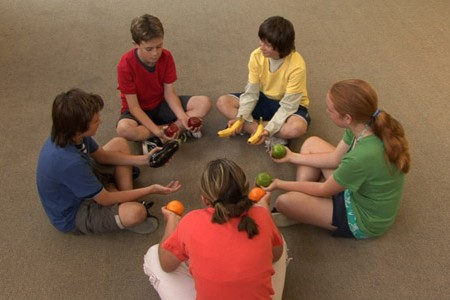
\includegraphics[width=100mm,scale=0.5]{images/orange-game.jpg}
  \caption{Déroulement du "Orange Game"}
  \label{fig:boat1}
\end{figure}

Ce que les enfants découvrent avec ce jeu, c'est que parfois on doit passer un fruit de sa propre couleur dans l'objectif de ne pas bloquer le jeu et de résoudre le problème. Ils sont donc sensibilisés à la mémoire tampon ou elle est ici représentée avec un emplacement libre sur un serveur ! Ils sont aussi sensibilisés à un problème de concurrence : l'interblocage. Ce problème peut donc être résolus en abandonnant un fruit de sa propre couleur.

Il est aussi possible d'introduire des notions comme le binaire aux enfants à l'aide de ces jeux. \cite{31} Par exemple, un des jeux du programme consiste à écrire son nom sur un bracelet en binaire, une lettre est codé avec 8 cases et les cases sont soit noires soit blanches (0 ou 1). On donne aux enfants la transcription des lettres en binaire et l'exercice est de faire la transcription de la feuille de code au bracelet. Ce jeu permet d'introduire aux enfants comment est fait la traduction sur les ordinateurs en partant du bit. Ceci bien sur après avoir expliqué aux enfants ce qu'était un bit, octet etc au travers du jeu. 

Un autre jeu pour découvrir le binaire est le "Binary numbers". \cite{32} Le but est de traduire des nombres décimaux en binaire ou l'inverse, par exemple 11000 en 24. Nous, nous savons qu'il faut faire quelque chose comme ${2^4 + 2^3}$ sauf que les enfants eux bien évidemment ne sont pas instruits aux notions de puissance mathématique, il faut donc réfléchir à une autre solution pour représenter les chiffres en binaire. Par conséquent l'idée du jeu est que 5 enfants se placent face à la classe et représentent chacun un bit. L'enfant a une pancarte en face de lui qui peut être retournée. De face la pancarte affiche un chiffre qui représente le 1 en binaire et de l'autre c'est une face noire qui représente le 0. Par exemple, si nous avons une disposition 10000, seul l'enfant à gauche aura sa pancarte côté face avec une valeur de ${2^4}$ sois 16 écrit dessus. Ce système apprend donc aux enfants à compter en binaire et à concevoir comment les chiffres sont traduits par un ordinateur.

\newpage

\begin{figure}[!htb]
  \centering
  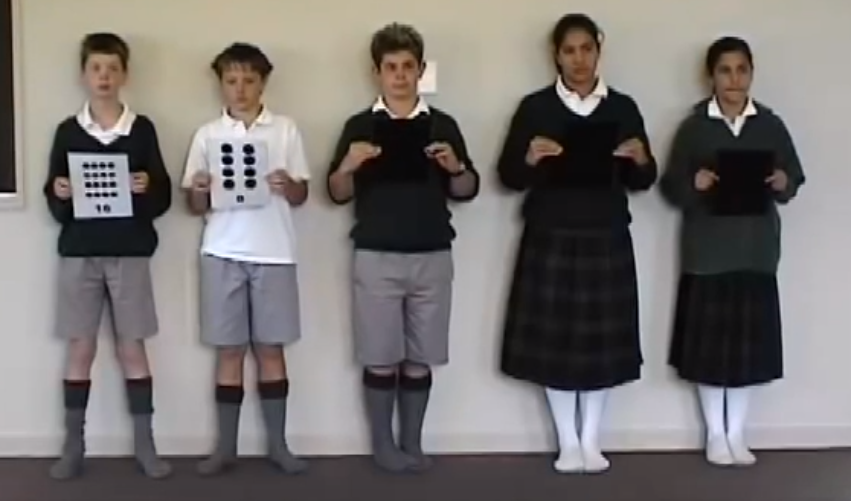
\includegraphics[width=100mm,scale=0.5]{images/binary-game.PNG}
  \caption{Représentation du 24 (11000) avec le Binary Game}
  \label{fig:boat1}
\end{figure}

Un dernier jeu que l'on peut citer du CS unplugged est celui des détections d'erreurs qui est donc une introduction à comment un ordinateur peut détecter et corriger des erreurs. Le principe est simple, on demande à un élève de disposer une grille 5x5 de cartes qui ont chacune une face noire et blanche (donc représentation de bits). L'élève dispose ses cartes en choisissant pour chacune la face qu'il souhaite. Le professeur ajoute ensuite une ligne et une colonne (nous avons donc une matrice 6x6). Le principe du jeu est qu'un élève change une des cartes de la matrice en la retournant et qu'un autre élève sache quelle case à été modifiée, sans avoir regardé le changement bien évidemment.

\begin{figure}[!htb]
  \centering
  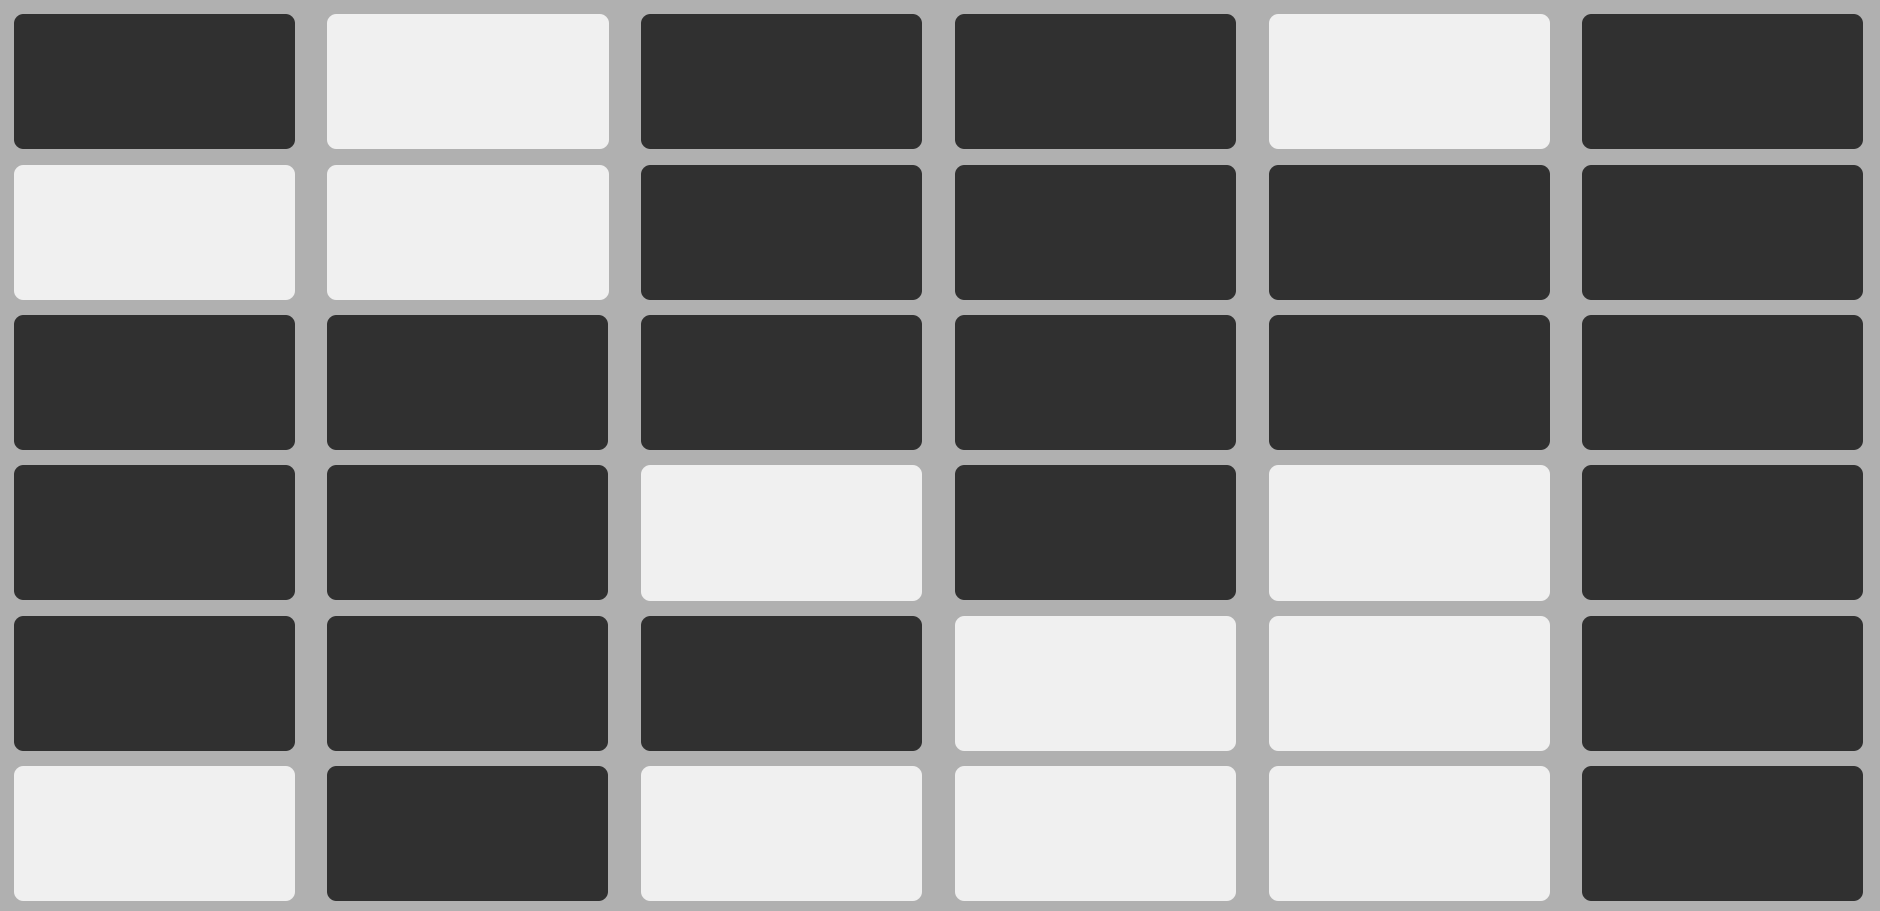
\includegraphics[width=70mm,scale=0.5]{images/error-detection.PNG}
  \caption{Exemple de matrice que l'on peut obtenir, source : \cite{33}}
  \label{fig:boat1}
\end{figure}

Comment, si on change une carte, peut-on deviner laquelle à été changée ? Quand on rajoute une ligne et une colonne ce n'est pas innocent, on fait en sorte que pour chaque ligne et colonne la couleur noire soit pair (4 noires première ligne, 4 noires première colonne etc...). C'est ainsi que si on change une carte on peut déterminer en comptant pour chaque ligne et chaque colonne quelle est la case incriminée. Une amélioration sur ce jeu pourrait notamment être expliquer pourquoi dans certaines cas les ordinateurs peuvent détecter une erreur mais pas la corriger ?

En conclusion, CS unplugged propose de bonnes idées pour aborder des concepts informatique sans avoir d'ordinateur. C'est une solution donc très accessible et gratuite. Cependant elle est tout de même critiquée. \cite{34} En effet, certaines activités semblent être plus difficile à associer à l'informatique que d'autres. Dans les cas d'exercices avec le binaire cela concerne directement le fonctionnement de la machine et c'est assez concret. Dans d'autres cas, comme avec le tri, il peut être plus difficile pour l'élève de faire le lien.

\newpage

Dans l'apprentissage manuel il existe aussi une solution pour les très petits (à partir de 3 ans). Ce sont tout simplement les jouets ! Il existe en effet des jouets destinés au codage qui peuvent demander à l'enfant de se poser des questions sur des sujets informatiques. \cite{39} Prenons un premier exemple avec le jouet "Code-a-pillar", accessible dès 3 ans qui permet d'assembler une chenille et faire en sorte qu'elle suive une sorte de programme définit par l'enfant.

\begin{figure}[!htb]
  \centering
  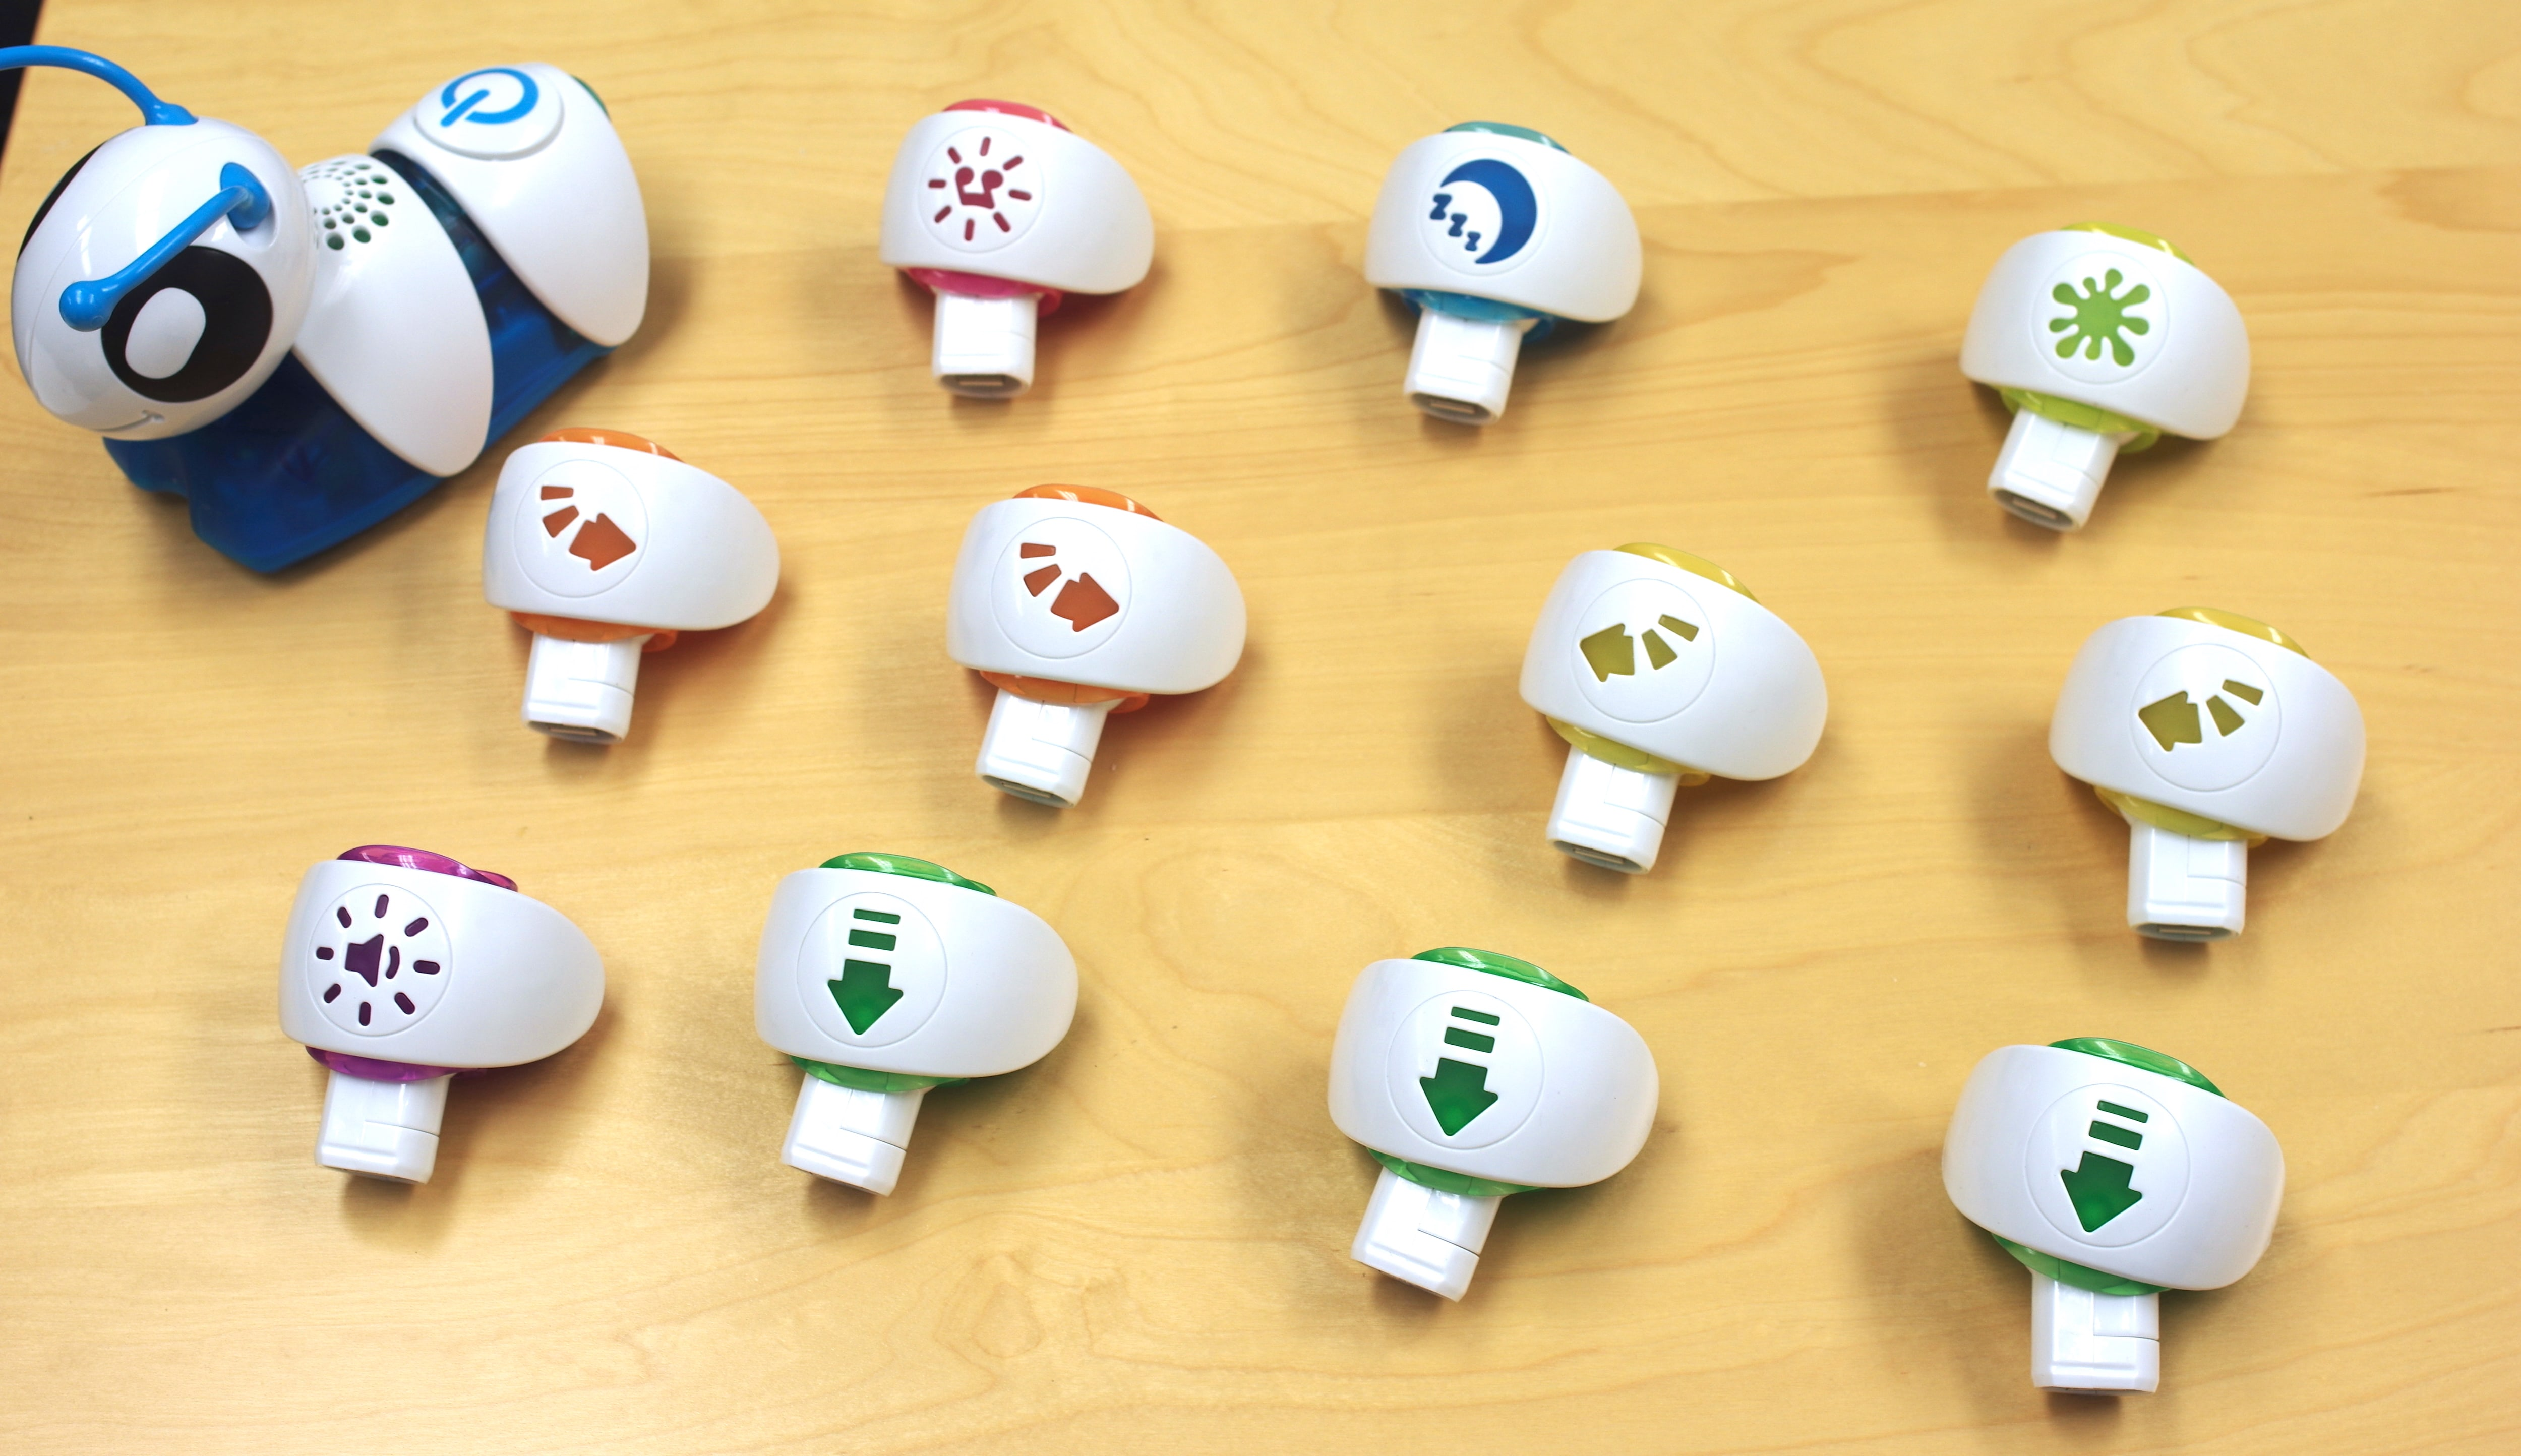
\includegraphics[width=85mm,scale=0.5]{images/codeapillar-min.jpg}
  \caption{"Code-a-pillar", le jeu de la chenille et ses pièces}
  \label{fig:boat1}
\end{figure}

Sur la figure ci dessus, nous avons les différentes pièces assemblables de la chenille. L'enfant choisit à sa guise les pièces et les met dans l'ordre qu'il souhaite. Ensuite, il appuie sur le bouton de mise en marche (le bleu qui lui est directement incrusté sur la chenille et qui ne peut pas être assemblé). La chenille se déplace ensuite selon le parcours que l'enfant a choisi. D'un point de vue informatique, chaque partie du corps de la chenille est une instruction et le corps entier est un programme que l'enfant à créé.

Un autre exemple, un jeu de carte "Potato Pirate", qui inclut des concepts d'ordre, d'instructions, conditions, boucles et opérateurs logiques. Dans ce jeu chaque joueur a une armée de patates et doit battre ses adversaires en éliminant leurs patates. C'est la méthode d'attaque (utilisant donc les concepts précédemment cités) qui est intéressante ! Un exemple ci-dessous avec deux boucles for imbriquées.

\begin{figure}[!htb]
  \centering
  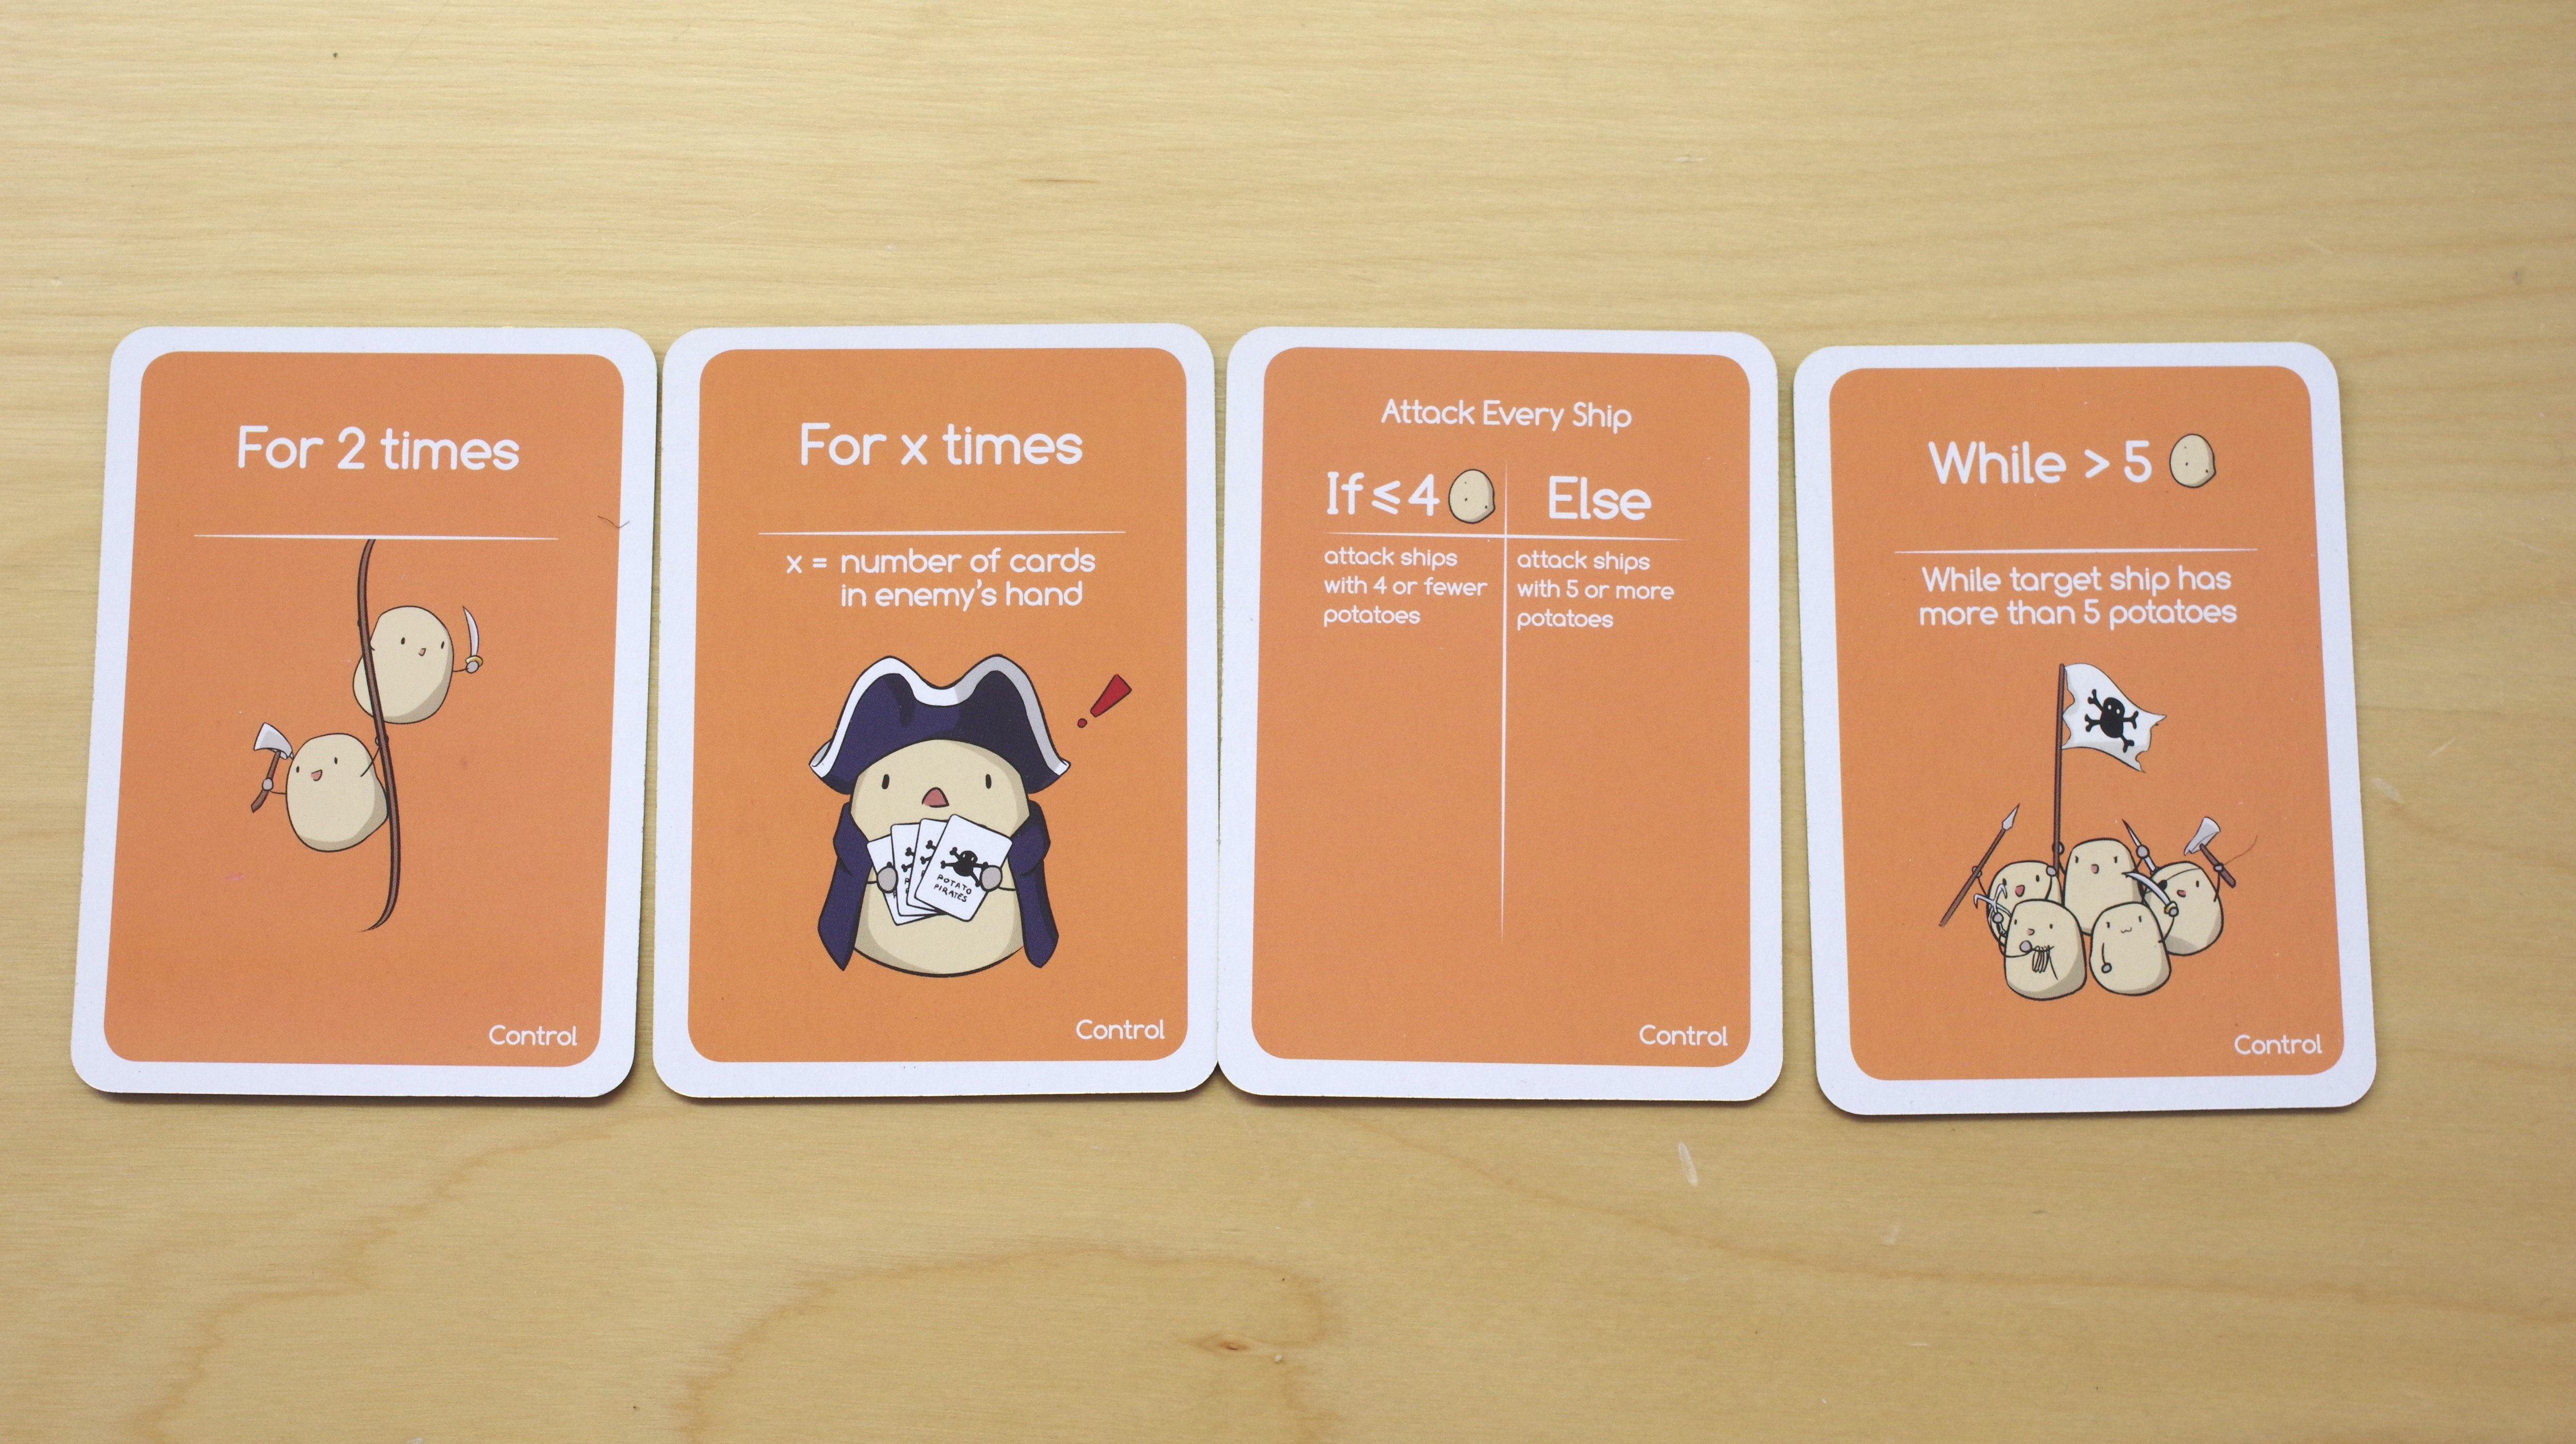
\includegraphics[width=110mm,scale=0.5]{images/control_cards-min.jpg}
  \caption{Exemple de cartes du jeu des patates}
  \label{fig:boat1}
\end{figure}

Contrairement au programme CS Unplugged, les jouets sont payants et sont en général destinés à la maison, pas en enseignement. De plus, il n'y a aucune étude qui vise à étudier les effets de ses jeux sur l'enfant, on peut cependant supposer que cela aide l'enfant à réfléchir d'une autre façon.

\newpage

\subsection{Les serious game}

Le serious game ou jeu sérieux a d'autres buts que le simple divertissement contrairement à un jeu vidéo. On peut énumérer l’enseignement, l’apprentissage, la communication, ou encore l’information qu'il vise à diffuser de manière ludique et pédagogique. Dans le cas de l'informatique, les jeux sérieux sont par exemple utilisés pour apprendre la programmation.

Les jeux sérieux ne sont pas adaptés pour les jeunes enfants (moins de 13 ans). Cependant ils peuvent être enseignés sans avoir eu de formation en informatique, cela dépend du jeu. Certains sont axés base de programmation et d'autres sont créés pour des langages spécifiques. Quand on parle de serious game la définition peut être ambiguë, on peut penser que par exemple Scratch ou Alice sont des jeux sérieux. Cette observation n'est pas fausse, cependant il y a différents niveaux de jeux sérieux, en général ils sont plus orienté programmation 'textuel' et non sous forme de drag-and-drop.

Est-ce que les serious game sont un bon moyen d'apprendre la programmation ? Donnons un exemple concret de serious game : CodeCombat \cite{38} CodeCombat est un jeu directement utilisable sur navigateur qui nous plonge dans un univers médiéval. On avance sur une sorte de plateau à la Mario Bros où chaque point est un nouveau niveau. Dans chaque niveau, un concept de programmation nous est présenté. L'avantage de CodeCombat est que le jeu a une visée éducative pour les enfants (visible sur leur site) et que toute la documentation y est présente pour accompagner les professeurs dans leurs démarches si ils souhaitent faire une expérimentation. Un autre avantage est qu'il est directement utilisable.

\begin{figure}[!htb]
  \centering
  \begin{minipage}[b]{0.48\textwidth}
    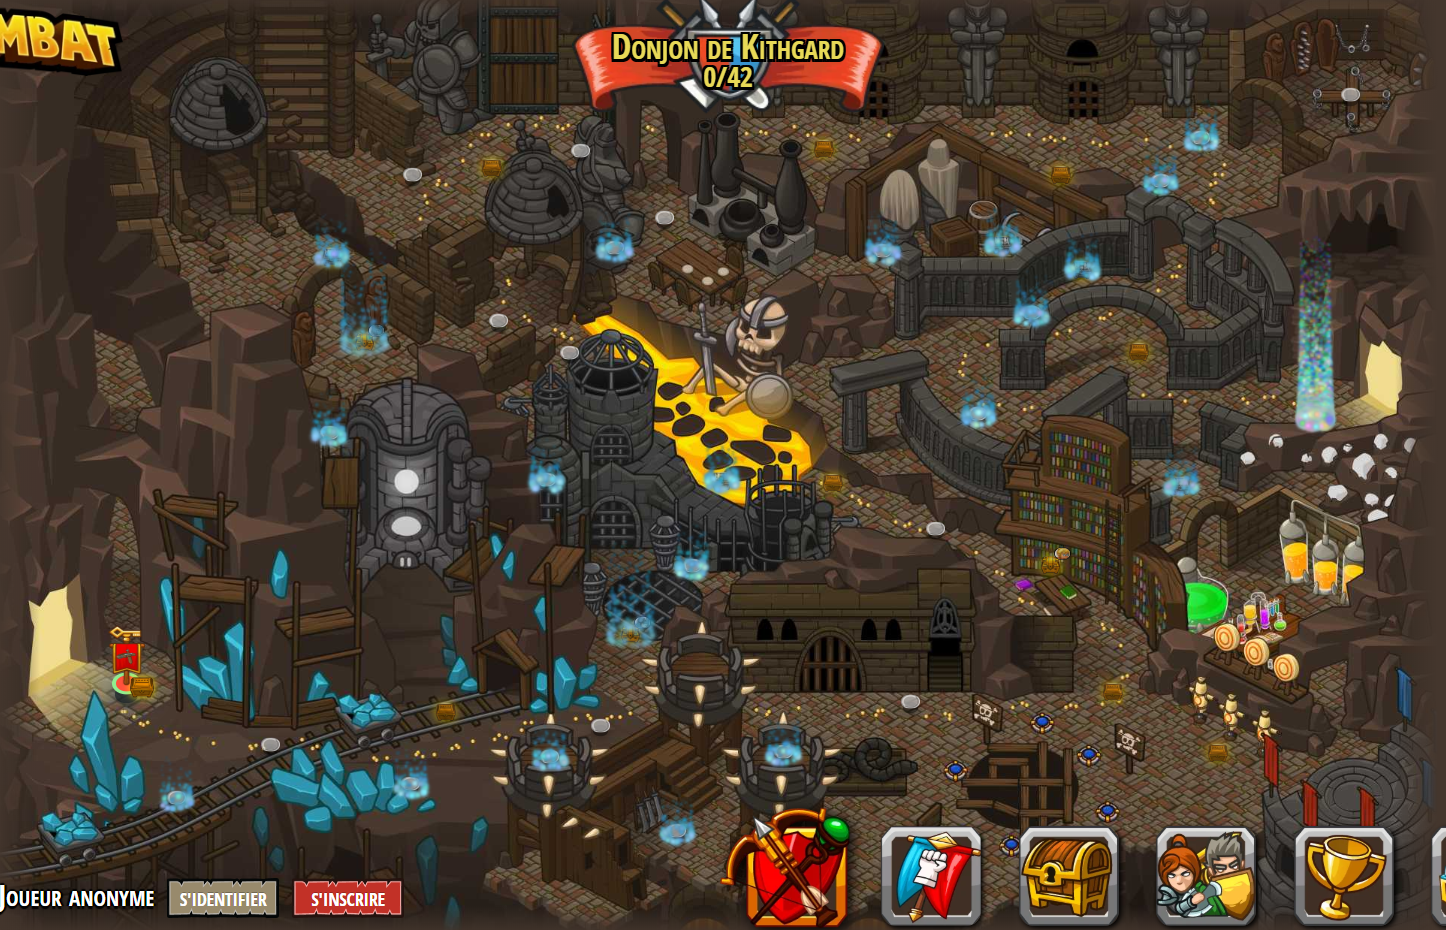
\includegraphics[width=\textwidth]{images/codecombat1.PNG}
    \caption{Plateau du jeu}
  \end{minipage}
  \hfill
  \begin{minipage}[b]{0.48\textwidth}
    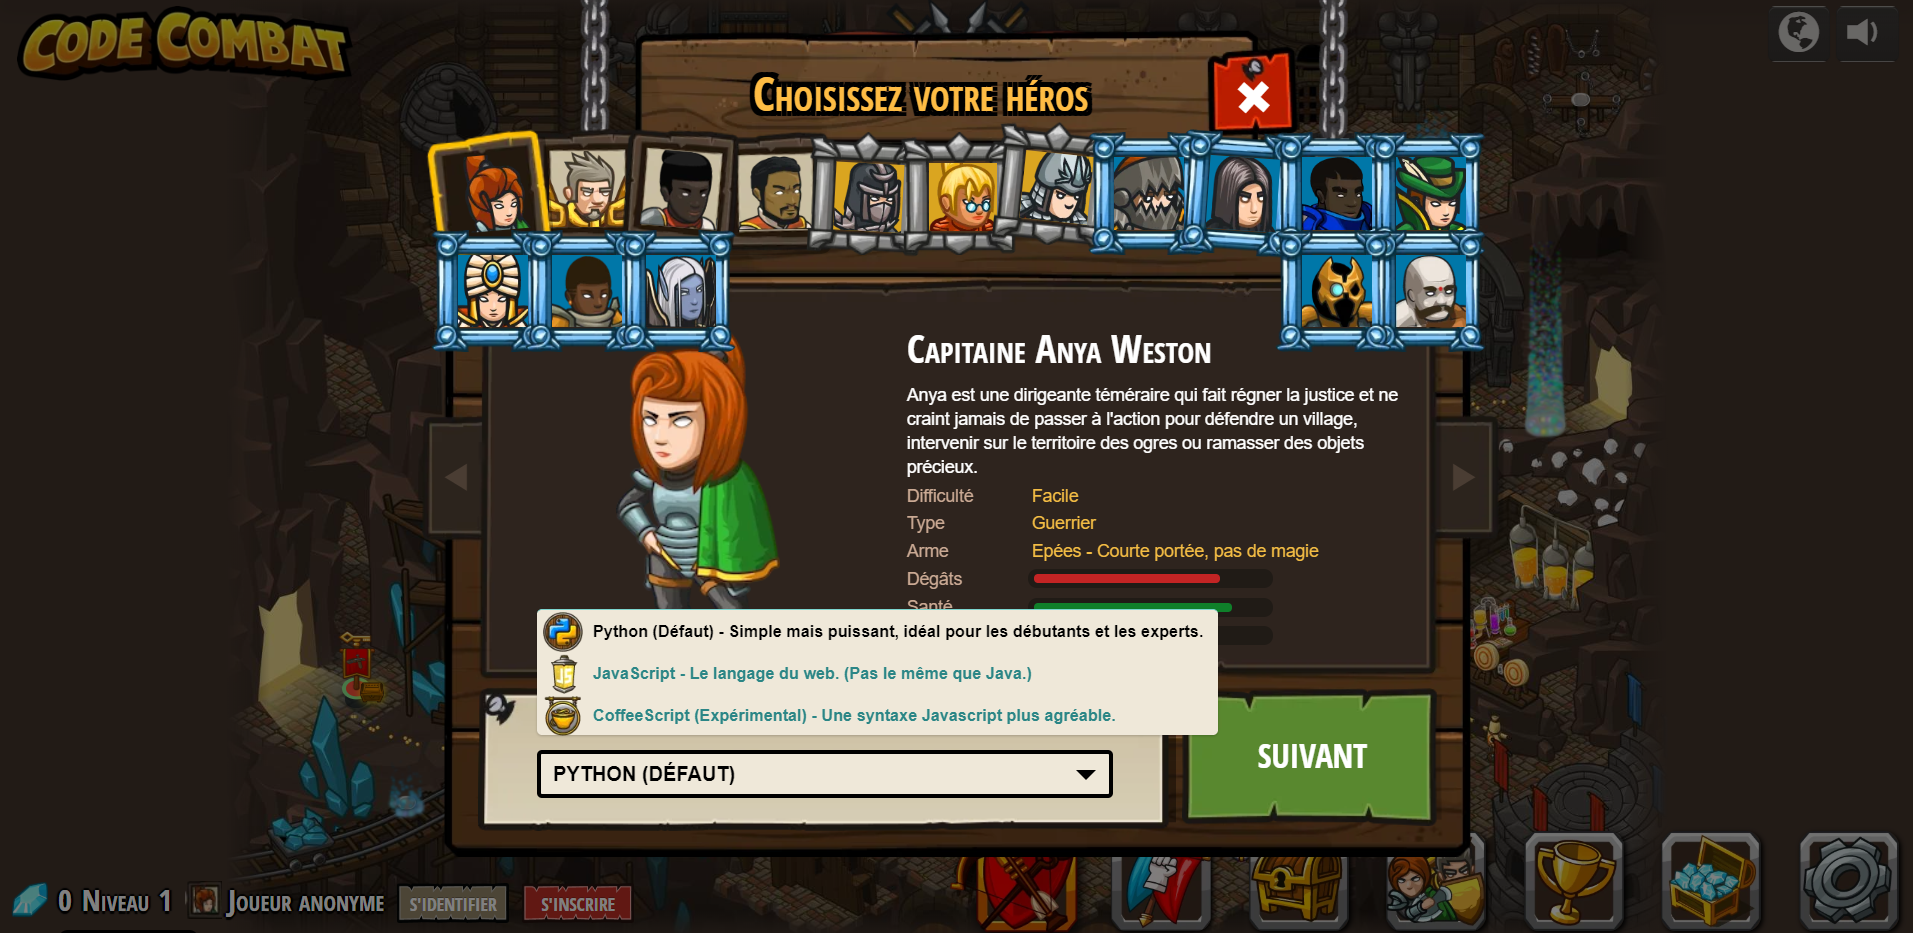
\includegraphics[width=\textwidth]{images/codecombat2.png}
    \caption{Paramètre du jeu, on a notamment le choix du langage}
  \end{minipage}
\end{figure}

L'interface est très ludique puisque on contrôle un personnage avec de la vie de l'attaque etc... Ce dernier a un équipement, doit combattre des ennemis, en bref on a l'impression d'être dans un vrai jeu vidéo. Cependant, contrairement à un jeu classique, ici les contrôles du personnage ne se font pas avec les croix directionnelles mais avec des instructions sous forme de ligne de code. On commence d'un état très basique ou les commandes pour déplacer le personnage ressemblent à : 

\begin{lstlisting}[frame=single]
hero.moveRight()
hero.moveUp()
hero.moveRight()
hero.moveDown()
\end{lstlisting}

Soit une syntaxe très simple car il n'y a aucun paramètre, pas de boucles etc... Juste une séquence d'instructions visant à appréhender la syntaxe basique d'un langage (qui est d'ailleurs ici le Python).

\newpage

À un autre état on apprend les paramètres, boucles, fonctions etc... On apprend même au joueur à bien lire la documentation des fonctions pour trouver la solution ou à utiliser des normes de programmation pour rendre le programme plus clair pour un lecteur extérieur. Il y a aussi la présence de gestion des erreurs du programme. Si on va plus loin dans le jeu on peut même voir des bonnes pratiques illustrées pour la réutilisabilité d'un programme etc... On peut notamment voir en annexe certains concepts qu'apprennent les niveaux suivants.

L'environnement assez riche de ce jeu et son interface intuitive fait que l'expérience éducative est assez addictive (notre personnage devient de plus en plus puissant, on débloque des instructions de code ...), nous sommes curieux de voir ce qu'il va se passer ensuite et la progression dans le code se fait de manière intelligente : la difficulté augmente de manière linéaire, toujours en lien avec les niveaux précédents. Le plus important, c'est que le jeu part du fait que l'utilisateur a un niveau zéro en programmation. Par conséquent, tout est bien expliqué en fonction de son niveau.

Le code est aussi très facilement testable car on voit directement l'action des instructions sur notre personnage. Si l'on a besoin de comprendre un nouveau concept, on peut alors s'essayer à changer des paramètres dans le programme pour voir l'effet que cela fait sur l'exécution. C'est un moyen très ludique pour apprendre.

\begin{figure}[!htb]
  \centering
  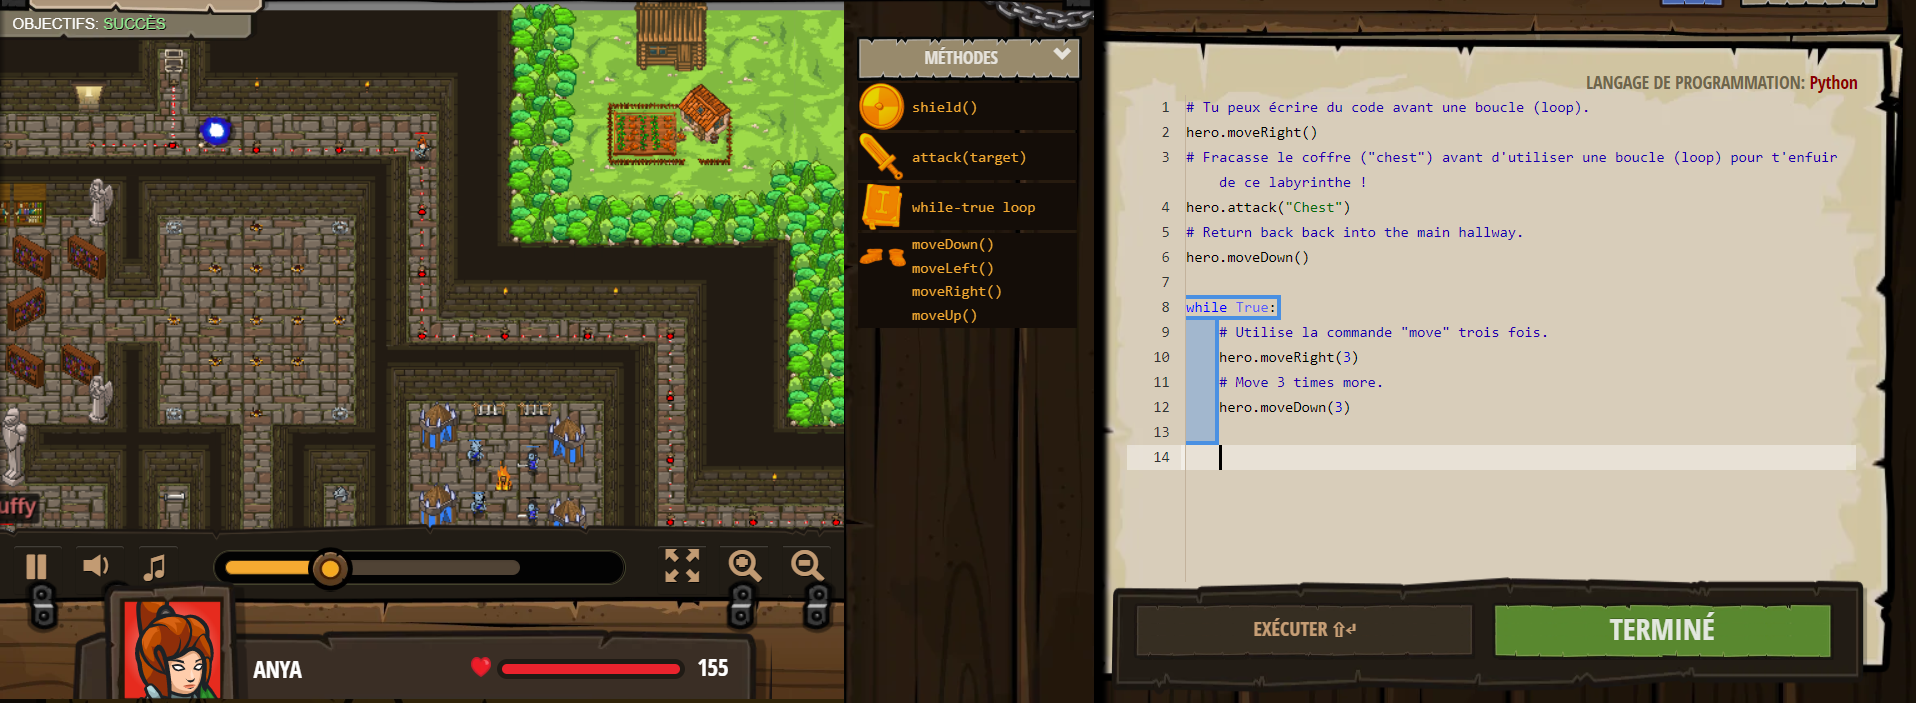
\includegraphics[width=150mm,scale=0.5]{images/codecombat4.PNG}
  \caption{Un niveau suivant et sa solution (environnement graphique à gauche et code à droite)}
  \label{fig:boat1}
\end{figure}

Un défaut de ce genre de solutions est cependant son prix, en effet seul les premiers niveaux sont gratuits, ensuite un inscription mensuelle ou à vie est requise.

Il existe de nombreux jeux sérieux commerciaux de ce genre. On observe notamment que plus souvent ces jeux sont basés sur des scénarios de jeux de fantaisies qui semblent correspondre donc à des enfants plus âgés en raison de la présence de combats, quêtes et d'une réflexion plus évoluée sur les concepts de programmation et la progression du jeu. Le marché de ces jeux est en constante augmentation et est victime d'un intérêt de plus en plus important. \cite{40} 

Même si tous les jeux ont leur propre particularité, que ce soit pour le langage à apprendre, la façon dont on est sensibilisé ou le niveau requis, le concept de l'apprentissage de la programmation par le jeu est récurrent. Ce que l'on peut se demander c'est : Est-ce que cette approche est efficace ? Les premières observations faites sur l'environnement de ces jeux sérieux tendent à montrer que c'est une solution efficace tant que les logiciels sont intuitifs et complets. Seulement, cela ne reste qu'une supposition.

\newpage

Des expérimentations ont été réalisées sur la création de jeux sérieux et le retour des élèves dessus. \cite{41} \cite{42} \cite{43} Même si ces études s'adressent parfois plus à un contexte de début de vie universitaire (les étudiants découvrent alors l'informatique avec les jeux sérieux dans un premier temps), il est tout de même intéressant de noter que dans la création d'un jeu sérieux l'environnement prends une place primordial car c'est bien évidemment ce dernier qui définit l'attractivité du produit. Une attention toute particulière est donc faite au contexte du jeu selon les tendances de jeu (plateforme, RPG, action etc) et un gros travail est aussi fait sur l'expérience utilisateur et la progression. Bien évidemment, un point essentiel du travail de développement est fait sur la pédagogie de l'informatique et de la programmation.

Dans les papiers de recherche, il est critiqué le fait que l'on reste en surface de l'univers de la programmation et que nous ne l'appliquons pas à un cas concret. Dans l'idée ou l'on apprend ces jeux sérieux à des élèves d'informatique débutant c'est une critique légitime. Dans un cas ou le jeu sérieux vise des enfants le plus important est que l'enfant intègre une façon de penser informatique et non pas qu'il devienne informaticien. 

Une autre observation, est que les étudiants ayant déjà programmé s'ennuyaient sur le jeu et le trouvait facile (c'est d'ailleurs la même observation que j'ai faite sur CodeCombat). En effet, pour des personnes déjà sensibilisé à l'informatique les jeux sérieux ne présente pas un énorme intérêt. Cependant, nous n'avons pas le recul nécessaire pour voir l'impact de cet apprentissage sur de parfaits néophytes de la programmation. Des observations que l'on en ressort, les néophytes trouvaient eux le jeu difficile et mettaient du temps à parcourir les niveaux, ce qui est intéressant car cela prouve l'utilité de ces jeux. Si ils mettent du temps à faire les niveaux contrairement à d'autres c'est qu'il doivent engranger du savoir et des façons de penser. En général les étudiants participant à ses recherches gardent une idée positive de la démarche. Les jeux sérieux permettent de susciter l'intérêt sur quelque chose qui peut être rebutant aux premiers abords (programmation). 

Une critique que l'on pourrait cependant faire, c'est que l'on n'a pas de données claires comme on avait pu l'avoir pour Alice ou Scratch, à savoir quelles sont les concepts de programmations acquis par l'utilisateur après expérimentation du jeu sérieux. Sur Scratch par exemple, il est possible à partir d'un projet d'exporter directement des statistiques sur l'utilisation de boucles, fonctions etc... grâce à une fonctionnalité incorporée sur le logiciel. C'est à dire que, à partir d'un projet on peut observer que l'enfant a vu certaines notions en fonction des briques de programmation qu'il a utilisées. Pour le cas des jeux sérieux nous n'avons pas concrètement les données mais il est évident qu'on peut déduire des notions apprises en fonction de la validité des niveaux. Dans CodeCombat on a notamment un suivi ou une note sur les étapes du jeu selon que notre code était "propre" ou non (nombre de lignes de code, le refactoring etc...). De plus pour chaque niveau est associé des concepts clairement énoncés.

Concernant mon expérience personnel sur différents jeux sérieux que j'ai pu tester, j'ai trouvé que le jeu était très guidé et empêchait la créativité comme on a pu le voir pour un Logo, Scratch, Alice etc... Étant donné que j'ai fait personnellement de l'informatique pendant 5 ans je n'ai peut être pas assez de recul nécessaire, mais peut être qu'un étudiant peut ne pas avoir assimiler certains concepts si il suit seulement les règles qu'on lui demande sur le jeu sans vraiment y réfléchir (on copie colle les exemples etc). Une autre observation est que, étant donné qu'en général ces logiciels sont des logiciels commerciaux, nous avons énormément d'informations que je trouve inutiles en rapport avec la communauté, les offres commerciales, les pop-up qui peuvent polluer l'expérience de jeu.

Le serious game est un concept intéressant car il suscite l'intérêt à l'informatique de façon ludique et permet son accessibilité. Cependant à part les projets de recherche et qui part définition n'ont pas les fonds pour faire un développement approfondi, les solutions de jeux sérieux sont payantes. On peut cependant espérer que les institutions éducatives payent des licences pour les élèves dans le cadre de cours introductifs à la programmation/informatique.

\newpage

\subsection{Les solutions extra-scolaires}

Comme pour la gymnastique, le club d'échec ou bien encore le centre de loisir, l'informatique a aujourd'hui ses ateliers extra-scolaires qui permettent aux parents d'inscrire leurs enfants de façon hebdomadaire ou dans un stage à des activités en rapport avec l'informatique ! Nous allons prendre un cas concret avec "Tech Kids Academy" implanté à Paris et à Saint-Germain-En-Laye. \cite{44}

Tech Kids Academy propose différents abonnements (stage, ateliers hebdomadaires) toujours dans le thème informatique. Affiché sur le site, nous avons la présence de technologies comme Scratch, Piskel, mais aussi des familiarisations à l'utilisation de robots comme par exemple avec Ozobot \cite{45} . Ici, on se rapproche de l'apprentissage manuel mais cependant avec Ozobot, on a également une interface sur ordinateur qui nous permet de faire des assemblages du style drag-and-drop comme avec un Scratch. Ces technologies étant plutôt simples d'utilisation elles sont adressées aux 7-9ans avec comme but je cite : "\textit{S’initier à la programmation créative, s’amuser avec des robots et découvrir l’électronique et la 3D}"

Nous avons 2 autres échelons, les 10-12 : "\textit{Découvrir le monde de la création de jeux vidéo, programmer des robots et inventer des objets connectés}" ainsi que les 13-17ans : "\textit{Coder avec des langages scripting, utiliser des logiciels de pros et explorer l’univers 3D et Arduino.}"

Arrivé au dernier échelon on apprend les langages de programmations comme Python, C, C++, C\# ainsi que l'arduino. Chaque échelon a ses propres caractéristiques pédagogiques et possède ses outils. Certains outils peuvent par contre être présents sur plusieurs échelons comme Scratch. L'enseignement est encadré par une équipe de passionnés par l'informatique, adultes ou étudiants.

Je pense que le fait de sortir du cadre scolaire peut apporter encore plus de motivation et d'attention à l'enfant étant donné qu'il n'a pas la sensation d'être à l'école et de travailler. Les retours (bien que sur le site donc non objectif) sont plutôt positifs que ce soit pour les parents ou pour les enfants.

Dans ce cadre les technologies utilisées sont des supports que nous avons parfois déjà vus comme Scratch. Mais il est intéressant de voir que Tech Kids Academy ne propose pas seulement de programmer ou de travailler derrière un ordinateur, mais également d'avoir aussi un apprentissage manuel avec l'électronique ou les robots qui sont des étapes essentielles pour un enfant (surtout jeune) qui a besoin de découvrir aussi avec le toucher.

Il existe différents ateliers du même genre que Tech Kids Academy et bien évidemment ce sont des solutions payantes (de \EUR{595} à \EUR{945} pour une année). Le prix est justifié en raison des équipements mis à disposition pour les enfants (robot, ordinateur, logiciel, accompagnement). Il faut aussi noter que ce genre d'ateliers sont transposables à l'école primaire. C'est notamment le cas pour Zenika en France \cite{46} avec des ateliers sur Scratch et sur les robots dans les écoles primaires sur une durée de un mois et demi. Cela à été réalisé sur l'année scolaire 2018 avec la complicité des enseignants et ils comptent bien continuer en 2019 en fonction des retours positifs qu'ils ont eu sur cette expérience.

%\begin{figure}[!htb]
%  \centering
%  \includegraphics[width=73mm,scale=0.5]{images/techkidacademy.jpg}
%  \caption{Salle de classe Tech Academy}
%  \label{fig:boat1}
%\end{figure}

\newpage

\subsection{Apprendre à la "dure" ?}

Une autre solution est de tout simplement apprendre un langage de programmation avec des tutoriels disponibles sur internet. Il existe des sites spécialisés qui proposent l'apprentissage avec absolument aucune base informatique. C'est par exemple le cas de OpenClassroom (ex siteduzero). \cite{47} C'est personnellement sur ce site que j'ai commencé à me familiariser au langage C et aux principes de programmation durant mon lycée en autodidacte.

Néanmoins, bien que OpenClassroom développe des tutoriels assez bien expliqués et propose même un suivi sur son site sur l'évolution de son apprentissage, apprendre de cette façon implique plusieurs choses. Le public de ce genre de site est le plus souvent des étudiants ou même des professionnels en reconversion. Pour les autres qui seraient mineurs, ces derniers sont plus généralement des petits curieux cherchant à comprendre comment marche la programmation. Le bon point est que le site propose énormément de tutoriels et aujourd'hui certaines thématiques du site sortent même de l'informatique depuis l'internationalisation de ce dernier. L'utilisateur, si il n'a pas d'obligation peut s'orienter vers le langage qu'il souhaite découvrir. Les adolescents qui utilisent ce genre de site pour découvrir la programmation sont donc une minorité dans la population, cela prouve aussi qu'en utilisant cette solution ils sont motivés à apprendre ce domaine. Or, dans les exemples précédents de sensibilisation les enfants n'avaient parfois aucune idée de ce qu'était la programmation et les techniques servaient notamment à leur présenter le domaine et à se donner une idée de si ça peut leur plaire. Dans le cas de OpenClassRoom, nous avons un public déjà convaincu. Ces derniers ont une volonté d'apprendre, dans les exemple précédents on 'camoufle' l'apprentissage avec des moyens dérobés comme les jeux, l'interaction graphique etc... 

Par conséquent, il n'y a pas vraiment d'esprit ludique dans ces solutions mais par contre on va tout de suite dans la profondeur des choses. Si on est très motivé pour apprendre un langage on peut passer par ce genre de site. Toutefois, aucune équipe enseignante va suivre l'évolution de l'utilisateur en direct. Openclassroom propose cependant des systèmes de tuteurs mais c'est bien évidemment payant.

Un risque de ce genre de solution est aussi que la programmation peut devenir intimidante  voire même engendrer un mauvais ressentis si on baisse trop vite les bras. Même si le site fait en sorte de progresser dans le langage doucement, il nécessite quand même une grande attention pour certains chapitres et un investissement. L'apprentissage est en plus fait pendant le temps libre contrairement à d'autres solutions présentées qui se faisaient en classe ou dans une activité extra-scolaire.

Ce qu'on peut tout de même noter c'est que par exemple Openclassroom utilise le MOOC (massive open online course) traduit par formation en ligne ouverte à tous ou des professionnels et/ou spécialistes du domaine partagent donc leur savoir en vidéo accessible à tous. Ce genre de solutions donnent de bons résultats dans l'enseignement. \cite{48}

\newpage

\subsection{Solutions nécessitant des bases informatiques}

En ouverture de cet état de l'art, nous allons aborder quelques solutions ludiques qui nécessitent des compétences informatique. Cela montre que faire de l'informatique ludique n'est pas seulement pour les néophytes.

Nous pouvons parler dans un premier temps de Robocode, projet open source, \cite{49} qu'on peut classifier dans les serious game étant donné que son premier objectif est destiné à l'apprentissage de Java. Le but de ce jeu est de programmer les réactions d'un char miniatures afin de faire des combats contre d'autres chars d'autres joueurs (Voir figure 2.22). Ainsi, les joueurs vont créer une compétition entre eux pour faire la meilleure intelligence artificielle de char afin de battre l'autre joueur et anticiper au mieux ses réactions. C'est un projet distribué gratuitement et mis à jour régulièrement (dernière mise à jour datant de mai 2019). Les meilleurs joueurs ont notamment recours aux réseaux neuronaux et/ou aux statistiques dans leurs algorithmes. Robocode est notamment présent dans des compétitions à travers le monde en Inde, Irlande, Espagne ... La communauté est active sur les forums du jeu et sa documentation est disponible gratuitement.

Tout ces éléments font que Robocode est une solution qui possède des caractéristiques qui font qu'on a envie de continuer à jouer. Même si certains joueurs peuvent pousser la compétition plus loin que les autres, si l'on reste aux bases du projet il sert notamment à apprendre Java de façon divertissante. Robocode est notamment un moyen d'apprentissage par problème pour les chercheurs. \cite{50} Il en ressort aussi de cette recherche que les étudiants utilisant RoboCode développent des compétences d'analyse de code, de tests, d'implémentation ainsi que de l'esprit critique sur leur travail. Des exemples de robots sont disponibles sur le GitHub de RoboCode. \cite{51}

\begin{figure}[!htb]
  \centering
  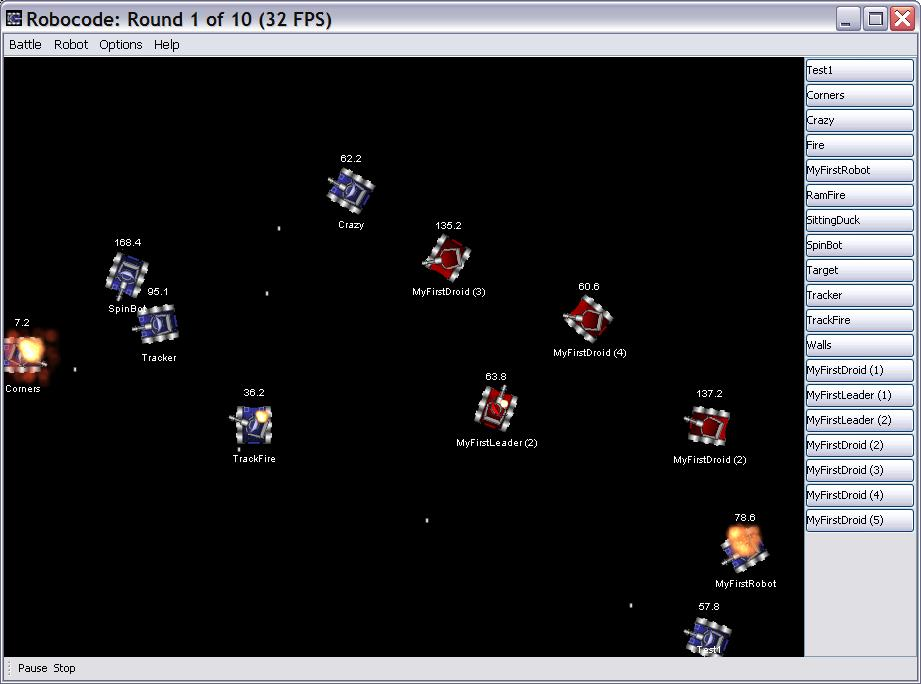
\includegraphics[width=80mm,scale=0.5]{images/robocode.jpg}
  \caption{Un combat RoboCode}
  \label{fig:boat1}
\end{figure}

On peut également parler de TIS-100, un jeu vidéo disponible sur des plateformes de jeux comme Steam. C'est un jeu de type puzzle où le but est de réaliser des tâches sur un vieil ordinateur des années 70 en assembleur. Même si cela n'est pas exactement de l'assembleur mais une copie, on retrouve quand même la complexité de travailler avec des langages de bas niveaux. Pour expliquer le jeu plus clairement, nous avons une interface avec plusieurs blocs dont certains peuvent être corrompus, il faut alors ré-écrire ces blocs pour réparer la machine. Nous utilisons alors les registres de la machines ainsi que des commandes comme MOV, JEZ, SWP, ADD, JMP. (Voir annexe) Si nous n'avons jamais programmé en assembleur, c'est un bon moyen d'avoir une vision de son fonctionnement avec le jeu vidéo. \cite{52}

\newpage

\section{Critique de l'existant et solutions envisagées}

En conclusion de cet état de l'art, nous pouvons déjà faire une remarque sur l'existant : il est très vaste. Je ne m'attendais pas à trouver autant de sources avant de commencer ce mémoire. Depuis 1967, avec Logo, différents projets ont émergé avec l'objectif d'apprendre aux enfants l'informatique de façon ludique. Avec les technologies actuelles, des logiciels très complets permettent également de faire avancer la recherche (comme avec Scratch par exemple et sa fonctionnalité de statistiques d'utilisation de briques). Cependant, on observe que malgré la présence de projets de laboratoire de recherches il émerge aussi des projets commerciaux comme avec les serious game ou bien les activités de loisir informatique. Chacune ont leurs avantages et inconvénients (gratuit, payant, suivi, addicitif, pédagogique, complet ...). Les solutions comme Logo sont très complètes étant donné que l'interface de programmation est un éditeur de texte. Nous ne sommes soumis à aucune interface graphique même si on crée du graphisme avec la tortue, les possibilités avec les primitives de Logo sont importantes. Dans les système drag-and-drop l'interface et les briques de code sont définies, certes,  cela n'empêche pas la créativité mais le cadre est plus restrictif. Cependant ces cadres restrictifs font que l'enfant est plus accompagné et qu'il peut être plus attentif aux cours et ainsi mieux apprendre. Il y a aussi des environnements moins clairs pour les enfants que d'autres. Finalement on peut toujours trouver des défauts et des avantages, l'important est que l'existant est important et que par conséquent il est plus facile de trouver un équilibre entre tous ces points dans une solution qui nous correspond.

Une remarque que l'on peut faire est que depuis des années les chercheurs et les entreprises ont créé des solutions pour enseigner l'informatique aux enfants. Par conséquent, pourquoi ce n'est pas ou en tout cas très peu (Voir Zenika et Scratch) abordé en France ? Comme déjà évoqué en début de mémoire, en France l'éducation nationale préfère peut être se focaliser pour ce qui est de l'école primaire des matières fondamentales comme la lecture et l'écriture qui est parfois non acquise même en fin de cycle. Cependant, nous avons déjà vu que l'informatique est un domaine intéressant tant il apprend à percevoir le monde, et nous permet de réfléchir d'une autre façon. \cite{53} Avec l'existant, pourquoi ne pas tenter un enseignement dans les collèges lycée ? Nous avons nous même vu que la formation des professeurs pour certaines solutions n'était pas importante (cela ne nécessite pas des compétences haute d'informatique mais plutôt de la logique).

Les solutions proposées, malgré leurs interfaces destinées à des enfants, comprenaient souvent des problèmes de compréhension de la part de l'enfant. Ce n'est pas forcément par rapport au logiciel en lui même mais par rapport aux instructions et leurs agencement (On a notamment observé cela en Logo ou avec Scratch et la compréhension des briques). On peut alors penser qu'un environnement déjà familier à l'enfant peut lui permettre d'encore mieux appréhender les concepts.

En conséquence des observations précédentes, nous allons penser à des solutions très simple d'accessibilité car elles se rattacheront à des connaissances de l'enfant ou seront dans un univers ludique. Ainsi elles seront transposables directement sans avoir à faire des installations compliquées. Si c'est un univers déjà connu pour l'enfant cela attisera sa curiosité et renforcera sa motivation. 

\newpage


\begin{table}[htb]
\begin{changemargin}{-3cm}{-3cm}
\resizebox{212mm}{40mm}{
\begin{tabular}{|l|l|l|l|c|c|c|c|c|c|c|c|c|}
\hline
Nom               & Type           & Public         & Cout    & \multicolumn{1}{l|}{Variable} & \multicolumn{1}{l|}{Séquençage} & \multicolumn{1}{l|}{Condition} & \multicolumn{1}{l|}{Boucle} & \multicolumn{1}{l|}{Fonction} & \multicolumn{1}{l|}{Récursivité} & \multicolumn{1}{l|}{Parallélisme} & \multicolumn{1}{l|}{Synchronisation} & \multicolumn{1}{l|}{Logique} \\ \hline
Doodle de Google  & Drag-And-Drop  & Jeunes enfants & Gratuit & \multicolumn{1}{l|}{}         & X                               & \multicolumn{1}{l|}{}          & X                           & \multicolumn{1}{l|}{}         & \multicolumn{1}{l|}{}            & \multicolumn{1}{l|}{}             &                                      &                              \\ \hline
Logo              & Langage/Dessin & Enfants/Ados   & Gratuit & X                             & X                               & X                              & X                           & X                             & X                                & \multicolumn{1}{l|}{}             &                                      &                              \\ \hline
HANDS             & Langage        & Enfants        & Gratuit & X                             & X                               & X                              &                             &                               &                                  &                                   &                                      &                              \\ \hline
Stagecast Creator & Jeu visuel     & Enfants        & Gratuit & X                             &                                 & X                              &                             &                               &                                  &                                   &                                      &                              \\ \hline
Visual Basic      & Langage        & Tous           & Gratuit & X                             & X                               & X                              & X                           & X                             & X                                & X                                 & X                                    &                              \\ \hline
Sonic Pi          & Langage        & Tous           & Gratuit & X                             & X                               & X                              & X                           & X                             & X                                & X                                 & X                                    &                              \\ \hline
Alice             & Drag-And-Drop  & Enfants        & Gratuit & X                             & X                               & X                              & X                           & X                             &                                  &                                   & X                                    &                              \\ \hline
Scratch           & Drag-And-Drop  & Enfants/Ados   & Gratuit & X                             & X                               & X                              & X                           & X                             &                                  &                                   & X                                    &                              \\ \hline
CS Unplugged      & Jeux           & Enfants        & Gratuit &                               &                                 & X                              &                             &                               &                                  & X                                 &                                      & X                            \\ \hline
Code-a-pillar     & Jouet          & Jeunes enfants & Payant  &                               & X                               &                                &                             &                               &                                  &                                   &                                      &                              \\ \hline
Potato Pirate     & Jeu de cartes  & Enfants/Ados   & Payant  & X                             & X                               & X                              & X                           &                               &                                  &                                   &                                      &                              \\ \hline
Code Combat       & Jeu sérieux    & Enfants/Ados   & Payant  & X                             & X                               & X                              & X                           & X                             &                                  &                                   &                                      &                              \\ \hline
Tech kids Academy & Atelier        & Enfants/Ados   & Payant  & X                             & X                               & X                              & X                           & X                             &                                  &                                   &                                      & X                            \\ \hline
RoboCode          & Jeu vidéo      & Tous           & Payant  & X                             & X                               & X                              & X                           & X                             & X                                & X                                 & X                                    &                              \\ \hline
TIS-100           & Jeu vidéo      & Tous           & Payant  & X                             & X                               & X                              & X                           & X                             &                                  &                                   &                                      &                              \\ \hline
\end{tabular}
}
\end{changemargin}
\caption{Tableau récapitulatif des solutions et des concepts qu'elles abordent}
\end{table}

Nous pouvons résumer avec le tableau ci-dessus une partie de l'état de l'art où nous associons à chaque solution ses caractéristiques. Nous pouvons faire l'observation cohérente que les solutions pour les plus jeunes enfants abordent moins de concepts comparé à d'autres qui touchent un public d'adolescents ou même d'adultes. Pour ce qui est de la logique, les solutions qui abordent ce concept sont celles qui donnent des pistes et des manières de raisonner avec de l'abstraction.

Souvent, les solutions qui abordent beaucoup de concepts demandent un investissement plus conséquent pour les appréhender. Celles qui abordent moins de concepts sont donc bien pour l'initiation. Comme nous avons vu avec  Stagecast, HANDS et Visual Basic nous pouvons apprendre des outils de plus en plus complexes pour un meilleur accompagnement de l'apprentissage.


\newpage

%%% Local Variables: 
%%% mode: latex
%%% TeX-master: "isae-report-template"
%%% End: 